\documentclass{article}

% Language setting
% Replace `english' with e.g. `spanish' to change the document language
\usepackage[italian]{babel}
\usepackage{color,soul}
\usepackage{cancel}

% Set page size and margins
% Replace `letterpaper' with `a4paper' for UK/EU standard size
\usepackage[a4paper,top=2cm,bottom=2cm,left=3cm,right=3cm,marginparwidth=1.75cm]{geometry}

% Useful packages
\usepackage{amsmath}
\usepackage{graphicx}
\usepackage[colorlinks=true, allcolors=black]{hyperref}

\title{Architettura dei calcolatori}
\author{Leonardo Donati}

\begin{document}
\maketitle
\tableofcontents

\newpage
\section{Introduzione}
Perchè è utile conoscere questa materia?
\begin{itemize}
    \item \textbf{Conoscere} il funzionamento
    \item \textbf{Ottimizzare} le prestazioni
    \item \textbf{Gestire} organizzazione che richiedono un sistema di calcolo
    \item \textbf{Progettare} architetture dei calcolatori delle prossime generazioni
\end{itemize}

\subsection{Tipi di architetture}
Ci sono più tipi di archietetture:
\begin{itemize}
    \item \textbf{General purpose:} ha almeno una CPU, un sistema operativo e gli applicativi sono scritti da terzi. Per esempio un computer normale.
    \item \textbf{Embedded:} può non avere un sistema operativo, hardware e software è tutto progettato.
    \item \textbf{Domain specific:} con specifiche ottimizzate per alcuni domini applicativi
    \item \textbf{High performance} progettate solo per applicazioni ad elevate prestazioni
\end{itemize}

\section{Definizione di Calcolatore Elettronico}
\hl{I calcolatori elettronici o computer si possono definire \textbf{sistemi digitali di elaborazione dell’informazione, programmabili e general-
purpose}.}

\subsection{Perchè sistema?}
Nell’ambito scientifico, un sistema è un qualsiasi oggetto di studio che, pur essendo costituito da diversi elementi reciprocamente interconnessi e interagenti tra loro o con l’ambiente esterno, reagisce o evolve come un elemento unitario, con proprie leggi generali.

\subsubsection{Come descrivere un sistema?}
Un sistema viene descritto attraverso il suo modello in uno specifico dominio di rappresentazione che indica l’insieme di particolari considerati di interesse. Per ogni livello si può fornire:
\begin{itemize}
    \item \textbf{Descizione funzionale:} descrive il funzionamento del sistema in termini di suoi ingressi e delle sue uscite.
    \item \textbf{Descrizione strutturale:} descrive la struttura in termini di elementi primitivi che lo compongono.
    \item \textbf{Descizione fisica:} descrive la effettiva realizzazione del sistema indicando in dettaglio i componenti impiegati e le loro interconnessioni.
\end{itemize}

\subsubsection{Descrizione funzionale}
Un sistema digitale che riceve in ingresso dati ed istruzioni e fornisce in uscita dati di risultati, ha, quindi, diversi compiti:
\begin{itemize}
    \item \textbf{Gestione delle istruzioni:} deve memorizzare, recuperare, interpretare ed eseguire le istruzioni di un programma per lavorare sui dati e controllare tutto il sistema.
    \item \textbf{Elaborazione dei dati:} deve elaborare dati binari.
    \item \textbf{Memorizzazione dei dati:} i dati prima e dopo della elaborazione devono essere memorizzati in modo temporaneo ed in modo permanente.
    \item \textbf{Trasferimento dei dati:} i dati devono essere trasferiti in ingresso ed uscita a sistemi direttamente collegati o deve essere instaurata una comunicazione con dispositivi remoti.
\end{itemize}

\subsubsection{Descrizione strutturale}
Descrive la parte hardware composta dai dispositivi fisici ed in particolare da una o più CPU (Central Processing Unit), da memorie e dispositivi di I/O collegati da uno o più bus e la parte software, costituita da software di base e software applicativo, ossia dai programmi che codificano in linguaggio macchina uno specifico algoritmo.

\subsubsection{Analisi (Reverse Engineering)}
\hl{L’analisi è lo studio del funzionamento di un sistema noto a
partire dalla sua struttura fino ad arrivare ad una sua descrizione
comportamentale (o funzionale).}

\subsubsection{Sintesi}
\hl{La sintesi di un sistema è al contrario il processo che porta alla
progettazione (e in seguito alla realizzazione) della struttura del
sistema, dei suoi componenti e delle connessioni tra componenti
a partire dalla descrizione comportamentale fino alla descrizione strutturale.}

\begin{figure}[!htb]
\centering
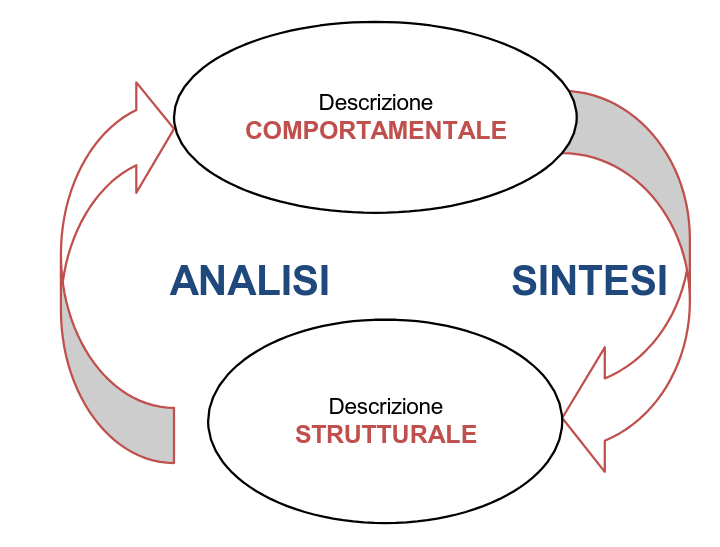
\includegraphics[width=0.35\linewidth]{Immagini/AnalisiSintesi.png}
\caption{Schema analisi e sintesi.}
\end{figure}

\subsection{Perchè programmabile?}
Un sistema che deve essere progettato o compreso viene definito ad un dato livello di astrazione.
Il livello di astrazione dell’architettura dei calcolatori è quello del programmatore di basso livello (o meglio del compilatore) e quindi l’architettura del calcolatore consiste nella struttura e l’organizzazione hardware delle parti e l’Instruction Set Architecture (ISA) ossia l’ insieme delle istruzioni, della struttura dei dati e dei meccanismi di controllo dei componenti.

\subsubsection{Astrazione}
\hl{Definire tutti i dettagli utili per comprenderne in dettaglio funzionamento o struttura ad uno specifico livello ignorando livelli di maggiore o minore dettaglio, e definendo interfacce per passare ai livelli maggiori o minori di astrazione.}

\subsubsection{Livelli di astrazione}
Il calcolatore è molto complesso, quindi viene studiato in diversi domini di rappresentazione e a diversi livelli di astrazione.
Per ogni progetto bisogna definire un modello, ossia astrazioni della realtà in cui si evidenziano aspetti di interesse e si sopprimono i dettagli non interessanti per il livello di astrazione in cui ci si collocano.
\newline\newline
\hl{Il livello di astrazione è quindi il grado di dettaglio del modello e la rappresentazione di quali sono i metodi per tradurre i dettagli in un livello di astrazione precedente o successivo.}

\newpage
\subsubsection{Livelli Hardware}
\begin{figure}[!htb]
\centering
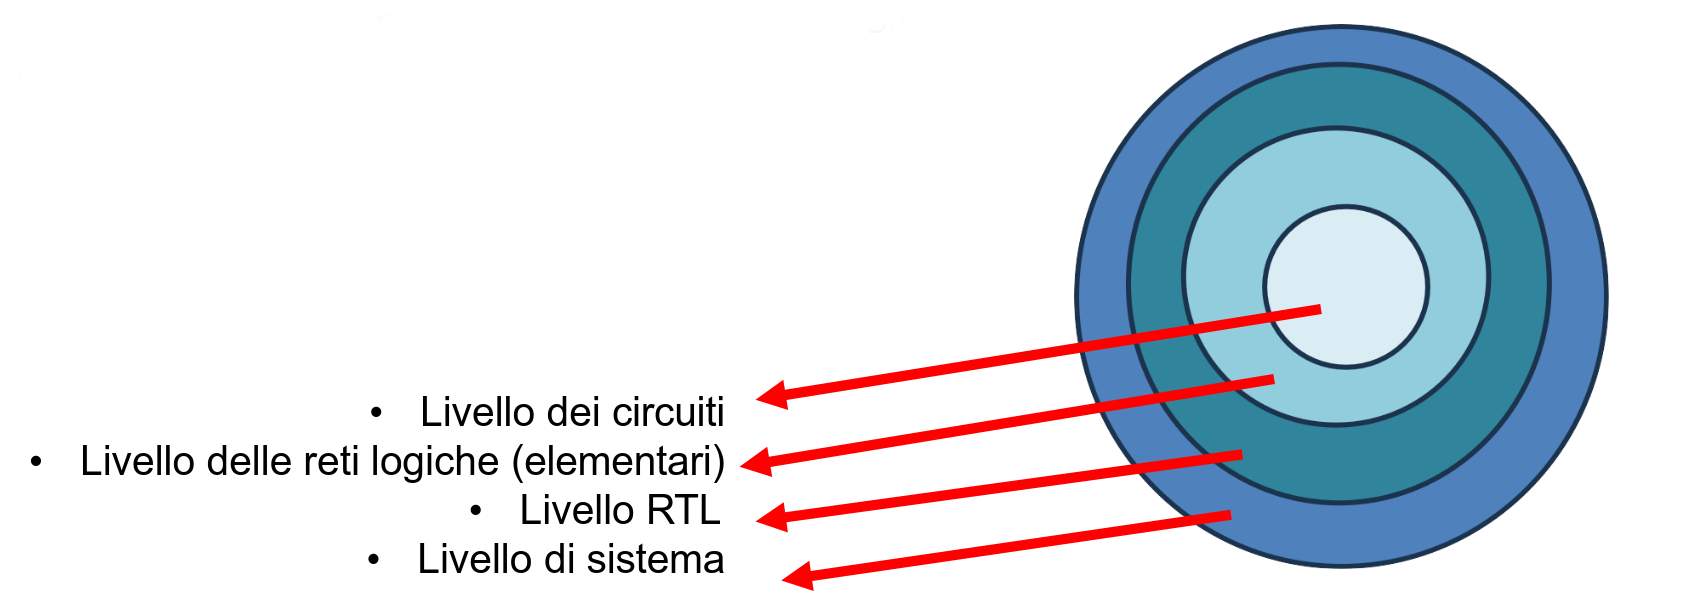
\includegraphics[width=0.80\linewidth]{Immagini/LivelliHw.png}
\caption{Livelli hardware di un calcolatore.}
\end{figure}
\begin{enumerate}
    \item \textbf{Livello dei circuiti}.
    \item \textbf{Livello delle reti logiche:} il cui linguaggio di descrizione è dato dal formalismo dell’algebra di Boole e degli automi a stati finiti.
    \item \textbf{Livello RTL(Registry transfer level):} i componenti che si descrivono si definiscono a livelli non di bit ma di parole, si usa un inguaggio formale RTL o linguaggi di descrizione dell’hardware (HDL Hardware description Languages).
    \item \textbf{Livello di sistema:} in cui si definiscono i componenti e le connessioni. Il linguaggio di descrizione è il linguaggio macchina, l’assembly e i linguaggi di programmazione come il C.
\end{enumerate}
I linguaggi di descrizione dell'hardware più usati sono il VHDL (VHSIC Hardware Description Language, dove VHSIC è la sigla di Very High Speed Integrated Circuits), oppure il SystemC.

\subsubsection{Livelli fra Hardware e Software}
Le funzioni che si possono ottenere con una sintesi hardware sono le stesse ottenibili in software e viceversa, con un diverso rapporto tra prestazioni e flessibilità. Per questo hanno in comune alcuni livelli: 
\begin{itemize}
    \item \textbf{Livello di microarchitettura:} è il livello che descritto come RTL o come sistema definisce le scelte sui blocchi logici che implementano la CPU e l’interno dei componenti del calcolatori.
    \item \textbf{Livello dell'ISA (Instruction Set Architecture):} Livello che definisce l’architettura della CPU e di conseguenza cio’ che il calcolatore puo’ svolgere. Ogni produttore ha un manuale della CPU e del proprio linguaggio Macchina implementato nell’ISA.
\end{itemize}

\subsection{Perchè digitali?}
Ogni calcolatore ha bisogno di dati digitali per compiere calcoli e processi.

\subsubsection{Dati}
\hl{I dati per un calcolatore sono tutte le grandezze quantificabili che vengono impiegate per un calcolo o per un processo.} Alcuni esempi possono essere numeri, lettere, valori grafici, audio e video.

\subsubsection{Differenza fra dati e segnali}
\hl{I segnali sono una qualsiasi grandezza fisica che varia nel tempo e che
può assumere un insieme di valori misurabili che possono essere trasmessi, memorizzati ed impiegati come dati in un computer.} Possono essere:
\begin{itemize}
    \item \textbf{Analogici:} se possono assumere infiniti valori all’interno di un dato intervallo.
    \item \textbf{Digitali:} se possono assumere un numero finito, discreto, di valori sempre all’interno di un dato intervallo di variabilità e quindi rappresentabile con numeri.
\end{itemize}
I segnali nascano normalmente nella natura di tipo analogico e sono acquisiti da sensori e trasformati in digitale attraverso convertitori.


\subsection{Perchè elaborazione dell'informazione?}
L’informazione, indipendentemente dal suo significato, può essere creata, ossia codificata, trasmessa ed elaborata in modo misurabile.
Il calcolatore elettronico ha il compito di elaborare l’informazione digitale.

\subsubsection{Informazione}
\hl{Si chiamano informazioni i dati che assumono un significato univoco, utile per una specifica applicazione. L’informazione è la riduzione di incertezza che si può avere a priori sul simbolo trasmesso.}

\subsubsection{Autoinformazione}
Ogni simbolo, di un alfabeto $ \text{X}=\{x_i,\space i = 1 \dots M\}$, $x_i$ avente probabilità $P(x_i)$ di essere trasmesso ha una informazione data dalla quantità, non negativa, definita come la riduzione di incertezza che si può stimare a priori sul simbolo trasmesso: 
\[I(x_i) = \log_B \frac{1}{P(x_i)}
         = -\log_B P(x_i)\]

\subsubsection{Entropia}
L’entropia è il contenuto informativo medio della sorgente o la misura della perdita di incertezza derivata, se si considera il valor medio, su tutto l’alfabeto dei simboli possibili, di $I(x_i)$:
\[H(x) = \text{E}[I(x_i)] = \sum_{i = 1 \dots M} P(x_i)I(x_i)\]
\\
\textbf{NB:} Dati M simboli: $0 < H(x) < \log M$

\subsection{Perchè digital purpose?}
I sistemi di elaborazione digital purpose hanno sempre determinate caratteristiche: 
\begin{itemize}
    \item Hanno sempre almeno una CPU.
    \item Dotato di sistema operatvio, software realizzato da terze parti.
    \item La sua funzionalità è specificata dal software applicativo.
    \item Può avere unità di elaborazione aggiuntive, come GPU, TPU, ecc...
\end{itemize}
Ci sono state diverse generazioni di calcolatori elettronici, in ognuna delle quali ci sono state evoluzioni e invenzioni importanti.

\subsubsection{Generazione 0}
Generazione 0 dei computer, il calcolatore era ancora un oggetto studiato tendenzialmente per risolvere calcoli matematici con elementi meccanici o elettromeccanici.

\subsubsection{Generazione 1}
La Generazione 1 dei computer però nasce con la nascita dell’elettronica e dei tubi a vuoto i precursori dei transistor, per creare la macchina ENIGMA per codificare i messaggi tedeschi e la macchina COLOSSUS parzialmente progettata da Alan Turing per decodificarli. 
Il modello attuale dei calcolatori deriva dal modello definito da Von Neumann negli anni ‘50.

\begin{figure}[!htb]
\centering
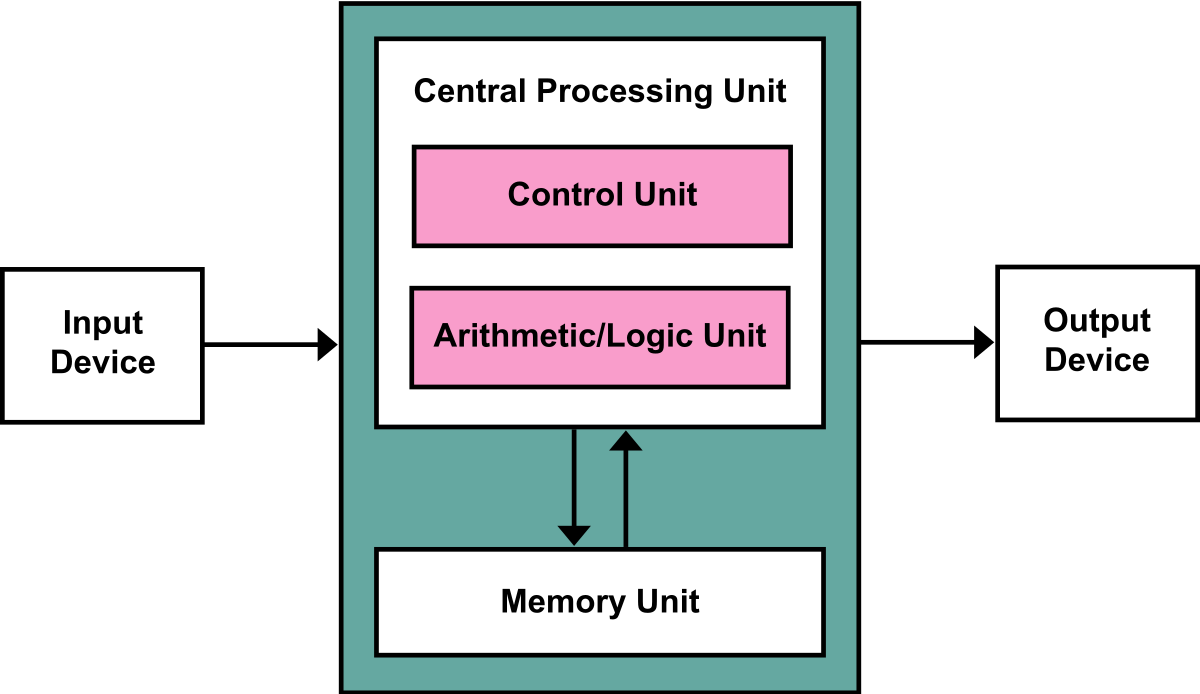
\includegraphics[width=0.35\linewidth]{Immagini/VonNeumann.png}
\caption{Architettura di Von Neumann.}
\end{figure}

\newpage
\subsubsection{Generazione 3}
Detta generazione dei circuiti integrati ('65-'70-'80), l’aspetto caratterizzante è la integrazione elettronica dei computer che da essere
grandi come stanze diventano di dimensioni più vicine a quelle dei calcolatori attuali.

\subsubsection{Generazione 4}
Nella 4° generazione o generazione dei VLSI (’80-), la larga scala di integrazione apre diverse possibilità a nuove forme di computers. Si sviluppano sempre più minicomputer accessibili anche a piccoli centri di calcolo che in assenza di internet hanno comunque accesso a dati e elaborazioni locali e possono collegarsi a reti mondiali sperimentali.

\newpage
\section{Prestazioni}
Conoscere come calcolare le prestazioni di tutto il calcolatore o della CPU e dei vari componenti è molto importante sia in fase di progettazione di un nuovo prodotto sia in fase di analisi e per la scelta, l’acquisto e l’uso di un calcolatore. In particolare, si parla di:
\begin{itemize}
    \item \hl{\textbf{Efficacia:} essere in grado di compiere il compito previsto.}
    \item \hl{\textbf{Efficenza:} la possibilità di svolgere il compito con minori risorse possibili.}
\end{itemize}
Nei calcolatori, le prestazioni dipendono molto dalla velocità, per questo è necessario analizzare diversi fattori:
\begin{itemize}
    \item \hl{\textbf{Tempo di esecuzione ($T_{exec}$):} tempo di esecuzione per un singolo task.}
    \item \hl{\textbf{Throughput:} quantità di task nell’unità di tempo.}
\end{itemize}

\subsection{Bottleneck}
\begin{itemize}
    \item \textbf{CPU-Bound} quelle applicazioni o programmi che sono limitate dalle prestazioni della CPU, tendenzialmente programmi di calcolo, di grafica, dove devono essere fatte molte operazioni di ALU e di memoria.
    \item \textbf{IO-Bound} quelle applicazioni o programmi che sono limitate dalle prestazioni delle periferiche di I/O, dai dischi anche distribuiti, dalla rete e dall’uomo; come ad esempio l’accesso ai Database o ai web server.
    \item \textbf{Memory-Bound} quelle applicazioni o programmi che sono limitate dalle prestazioni della memoria centale come in Database in-memory e come per l’addestramento di reti neurali di grandi dimensioni. Spesso si migliora con una architettura efficace delle cache.
\end{itemize}

\subsection{Tempo di CPU}
Il calcolo delle prestazioni con un modello analitico semplice si interessa solo della CPU:
\[T_{cpu} = Ncc \space\space T_{clk} = \frac{Ncc}{f}\] 
Dove: 
\begin{itemize}
    \item \textbf{Ncc} è il numero di cicli di clock.
    \item \textbf{$f$} è la frequenza di clock.
    \item \textbf{$T_{clk}$} è il tempo di clock.
\end{itemize}

\subsection{Clock per instruction (CPI)}
Numero di periodi di clock impiegati mediamente per eseguire una istruzione considerando un insieme di programmi, su una specifica CPU:
\[\text{CPI} = \frac{Ncc}{Ni} = \sum(x_i \space CPI_i)\]
Quindi, possiamo calcolare il tempo di CPU anche come:
\[T_{cpu} = Ni \space\space \text{CPI} \space\space T_{clk} = \frac{Ni \space\space \text{CPI}}{f} \]
Dove:
\begin{itemize}
    \item \textbf{Ni} è il numero di istruzioni.
\end{itemize}

\subsection{Speed Up}
\hl{Speedup o accelerazione e’ un indice di miglioramento di quanto e' migliorata la prestazione globale avendo migliorato una parte del sistema.} E’ il rapporto tra la prestazione ottenuta con il miglioramento rispetto a quella ottenuta senza miglioramento.
\[\text{SP} = \frac{T_{exec-old}}{T_{exec-new}}\]

\subsection{Legge di Amdhal}
Il miglioramento delle prestazioni dovute ad un miglioramento di esecuzione e' limitato dalla frazione di tempo in cui tale miglioramento puo’ essere applicato.
\[\text{SP(overall)} = \frac{1}{(1- F_{enh}) + \frac{F_{enh}}{S_{enh}}}
    = \frac{1}{[1- \sum_i(F_{enh_i})]+ \sum_i(\frac{F_{enh_i}}{S_{enh_i}})}
\]
Dove:
\begin{itemize}
    \item \textbf{$F_{enh}$(fraction enhanced)} è la percentuale di tempo in cui ha effetto il miglioramento.
    \item \textbf{$S_{enh}$(speedup enhanced)} è il valore di tale miglioramento.
\end{itemize}

\begin{figure}[!htb]
\centering
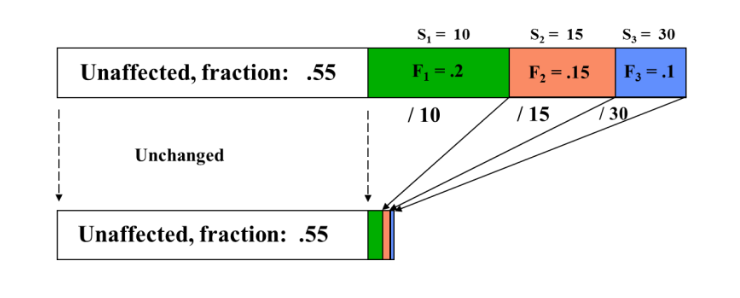
\includegraphics[width=0.60\linewidth]{Immagini/SpeedUpOverall.png}
\caption{Speed up effittivo di tre CPU.}
\end{figure}



\newpage
\section{Benchmark}


\newpage
\section{Reti logiche}
Il livello delle reti logiche è il livello di astrazione che studia i sistemi digitali a livello di componenti logici elementari, chiamati gate, indipendentemente dalla loro realizzazione fisica. Invece, dal punto di vista funzionale, \hl{la rete logica è la astrazione di un sistema digitale avente n segnali binari di ingresso ed m segnali binari di uscita ed una funzione logica che mette in relazione i segnali
di uscita con quelli di ingresso.}

\subsection{Rete combinatorie VS reti sequenziali}
Una rete è combinatoria se ogni segnale di uscita dipende solo dai valori degli ingressi in quell’istante, invece, una rete è sequenziale se ogni segnale di uscita dipende dai valori degli ingressi in quell’istante e dai valori che gli ingressi hanno assunto negli istanti precedenti.

\subsection{Algebra di Boole}
L’algebra di Boole è un sistema matematico che descrive funzioni di variabili binarie, composto da: 
\begin{itemize}
    \item Un insieme di simboli $\text{B}=\{0,1\}$.
    \item Un insieme di operazioni $\text{O}=\{+,\space\cdot,\space'\}$.
          \begin{enumerate}
              \item Somma logica $+$.
              \item Prodotto logico $\cdot$.
              \item Complementazione $'$.
          \end{enumerate}
    \item Un indieme di postulati(assiomi) P.
\end{itemize}

\subsubsection{Tabella di verità}
La Tabella di verità è una: tabella che associa tutte le possibili combinazioni degli ingressi alle corrispondenti configurazione delle uscite, e indica esaustivamente il comportamento della rete logica.

\begin{center}
\begin{tabular}{|c c c | c c c|} 
 \hline
 $x_1$ & $\dots$ & $x_n$ & $y_1$ & $\dots$ & $y_m$ \\
 \hline
 1 & $\dots$ & 0 & 1 & $\dots$ & - \\ 
 \hline
 0 & $\dots$ & 1 & - & $\dots$ & 1 \\
 \hline
 1 & $\dots$ & 0 & 1 & $\dots$ & 0 \\
 \hline
 0 & $\dots$ & 1 & 0 & $\dots$ & 1 \\
 \hline
 1 & $\dots$ & 0 & 1 & $\dots$ & - \\
 \hline
\end{tabular}
\end{center}

Una tabella di verità di $n$ variabili di ingresso ha $2^n$ righe. Si possono creare $2^{2^n}$ tabelle delle uscite.

\subsubsection{Funzioni logiche di una variabile}
Sono 4 possibili funzioni:
\begin{itemize}
    \item \textbf{Massa:} l'uscita vale sempre 0.
    \item \textbf{Buffer:} l'uscita è sempre uguale all'ingresso.
    \item \textbf{NOT o complementazione:} l'uscita è sempre l'opposto dell'ingresso.
    \item \textbf{Vcc:} l'uscita vale sempre 1.
\end{itemize}

\subsubsection{Funzioni logiche di due variabili}
Sono 16 possibili funzioni:
\begin{itemize}
    \item \textbf{AND:} l'uscita vale 1 se entrambi gli ingressi sono 1.
    \item \textbf{OR:} l'uscita vale 1 se almeno uno dei due ingressi vale 1.
    \item \textbf{XOR} l'uscita vale 1 se almeno uno dei due ingressi vale 1 ma non entrambi.
    \item \textbf{NOR} l'uscita vale 1 se entrambi gli ingressi sono 0.
    \item \textbf{XAND} l'uscita vale 1 se entrambi gli ingressi sono diversi da 1.
    \item \textbf{XNOR} l'uscita vale 1 se gli ingressi sono uguali.
\end{itemize}

\subsubsection{Proprietà di interconnessione}
L’interconnessione di più reti logiche, aventi per ingresso segnali esterni o uscite di altre reti logiche e per uscite segnali di uscita esterne o ingressi di altre reti logiche, è ancora una rete logica.

\subsubsection{Proprietà di decomposizione}
Una rete logica complessa può essere decomposta in reti logiche più semplici.

\subsubsection{Altre proprietà}
\begin{figure}[!htb]
\centering
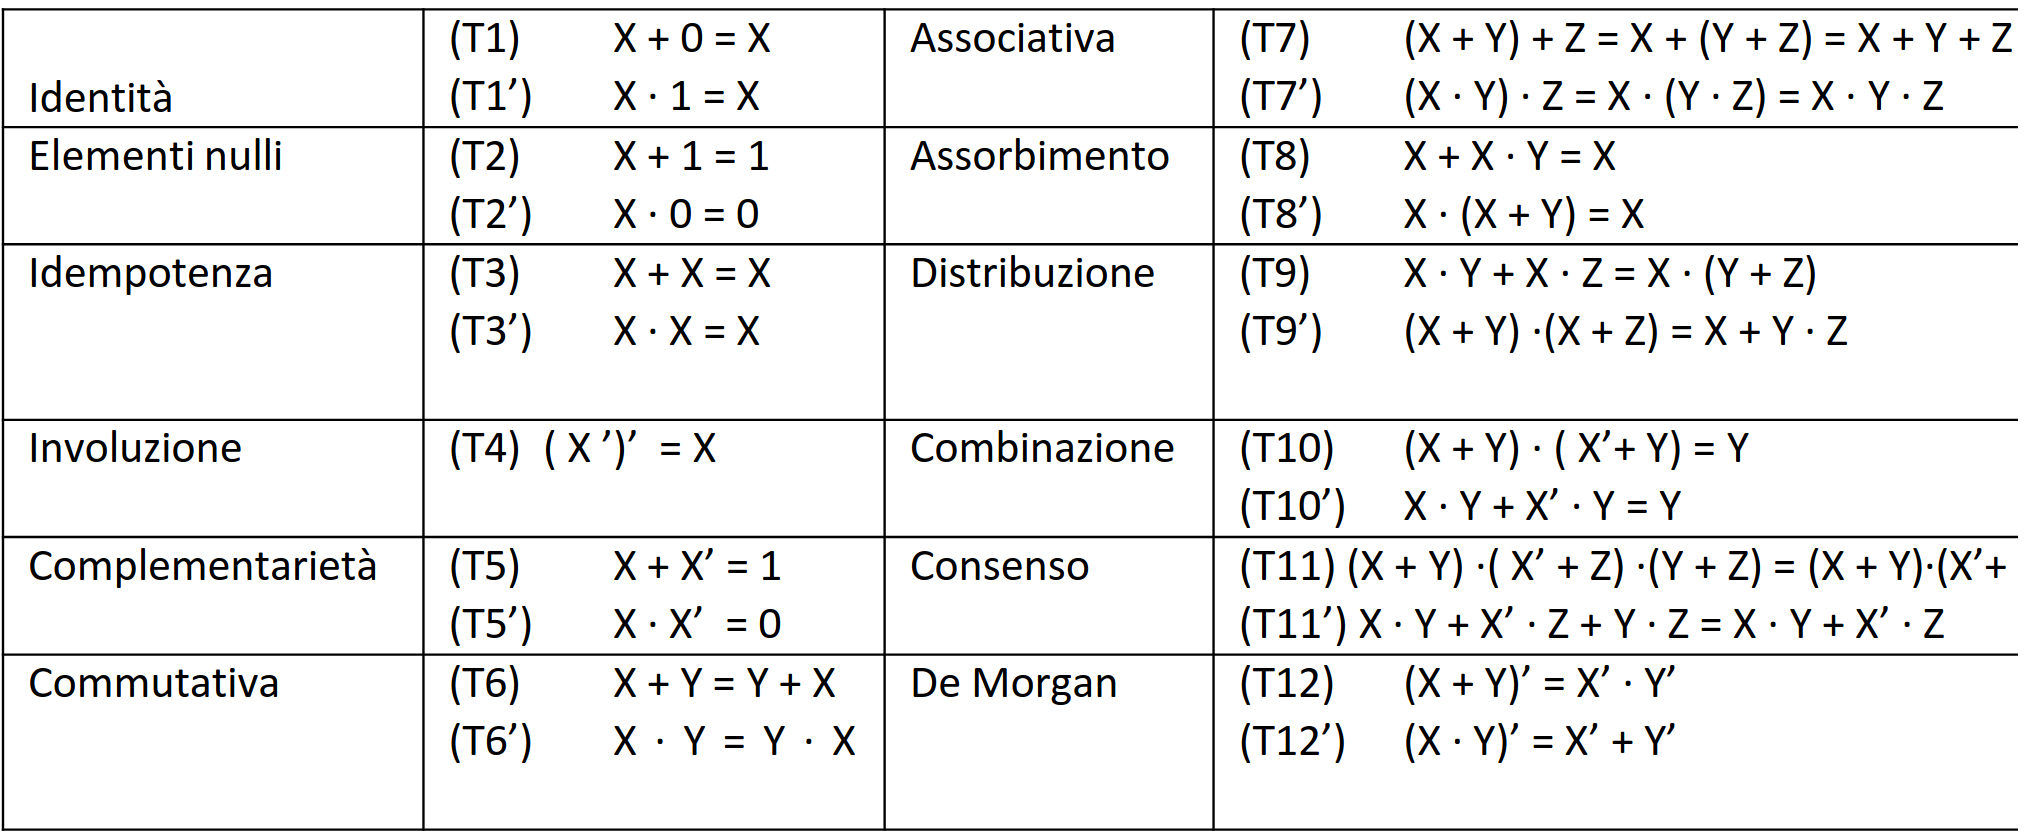
\includegraphics[width=0.80\linewidth]{Immagini/Proprietà.png}
\caption{Altre proprietà algebra lineare.}
\end{figure}

\subsubsection{Mappe di Karnaough}
Deve rispettare la distanza di Hamming, ossia le configurazioni di bit adicenti non devono differire per più di un bit.
\begin{figure}[!htb]
\centering
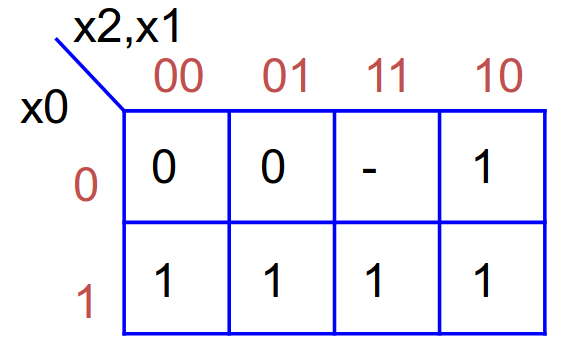
\includegraphics[width=0.50\linewidth]{Immagini/Karnaough.png}
\caption{Esempio di mappa di Karnaough.}
\end{figure}

\subsubsection{Letterale}
Sia dato un circuito combinatorio con n variabili di ingresso, X:$ \{X_1..X_n\}$. \hl{Si chiama letterale ogni occorrenza di una singola variabile, sia in forma semplice $X_i$ che complementata $X_i'$.}
Se abbiamo Z= ABC+AB’, allora A, B,B’ e C sono letterali della funzione.

\subsubsection{Implicante}
\hl{Si dice implicante di una funzione $f(X_i,\space\dots, X_n)$ un prodotto $P(X')\space\text{con}\space X'\subseteq X$ di letterali tale che $P=1 \implies f=1$.
Si chiama implicante primo di una funzione $f$ un implicante di $f$ che non è coperto da un altro implicante di $f$ con meno letterali.}
Gli implicanti e gli implicanti primi si possono vedere nelle mappe di Karnaugh dove i raggruppamenti rettangolari che coprono le uscite pari a 1, indicano gli implicanti e gli implicanti primi se non esistono altri raggruppamenti rettangolari che li coprono.

\begin{figure}[!htb]
\centering
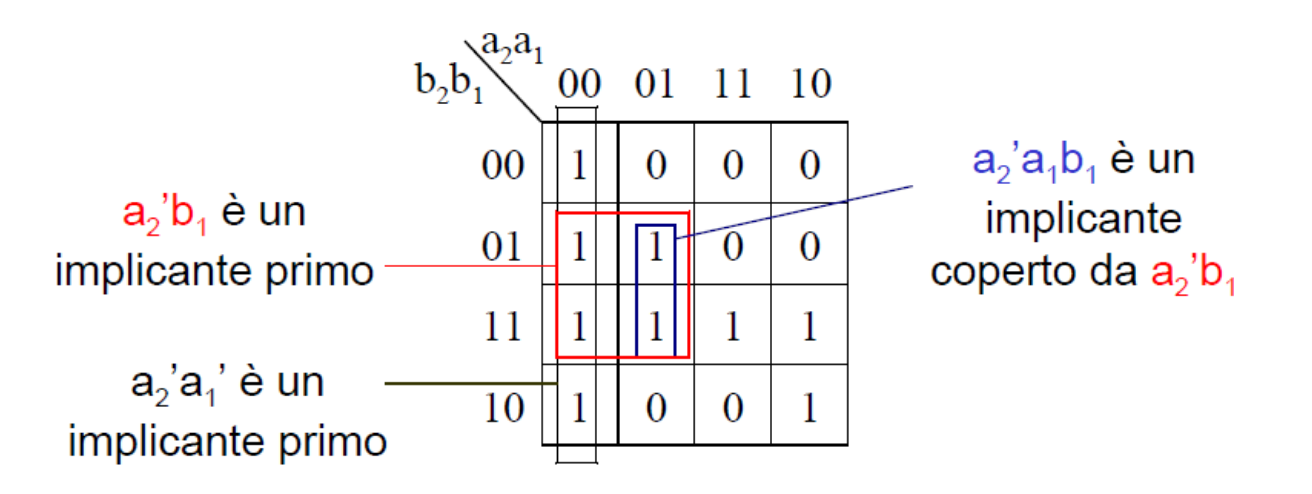
\includegraphics[width=0.70\linewidth]{Immagini/KarnaoughImplicanti.png}
\caption{Esempio di implicanti nella mappa di Karnaough.}
\end{figure}

\subsubsection{Mintermine}
La funzione che prende il nome di prodotto fondamentale (o mintermine) è costituita dal prodotto logico dei letterali delle variabili di ingresso, presi negati se nella riga considerata la corrispondente variabile di ingresso vale 0, non negati se tale variabile vale 1.
\\
\hl{Si definisce mintermine di una funzione $f(X_1, \space\dots, X_n)$ un punto $B_x$ nello spazio booleano $B_n$ tale per cui $f(B_x)=1$.}

\subsubsection{Maxtermine}
La che funzione prende il nome di somma fondamentale (o maxtermine) è costituita dalla somma logica dei letterali delle variabili di ingresso, presi non negati se nella riga considerata la corrispondente variabile di ingresso vale 0, negati se tale variabile vale 1. 
\\
\hl{Si definisce maxtermine di una funzione $f(X_1, \space\dots, X_n)$ un punto $B_x$ nello spazio booleano $B_n$ tale per cui $f(B_x)=0$.}

\subsubsection{Sintesi canonica}
La sintesi canonica non è minima ma può essere minimizzata con diversi algoritmi tra i quali quelli che impiegano la semplificazione algebrica.
La sintesi canonica ha però il vantaggio di garantire la massima velocità dato che impiega due livelli di gate S e P o P ed S, ed inoltre permette il riuso degli elementi logici se si devono realizzare piu’ reti logiche con gli stessi ingressi. Non è necessario quindi cercare per forza la sintesi minima.
\begin{itemize}
    \item \textbf{Sintesi canonica SP (Somma di prodotti):} una funzione di n variabili può essere espressa in un solo modo come somma di prodotto di n variabili, ossia di mintermini.
    \item \textbf{Sintesi canonica PS (Prodotto di somme):} una funzione di n variabili può essere espressa in un solo modo come prodotto di somme di n variabili, ossia di maxtermini.
\end{itemize}

\newpage
\subsection{Multiplexer}
Seleziona un singolo input fra diversi segnali in ingresso, in base al valore degli ingressi (dell’ingresso) di selezione.
Data la tabella:
\begin{center}
\begin{tabular}{|c c c | c |} 
 \hline
 A & B & S & Y \\
 \hline
 a & * & 0 & a \\
 \hline 
 * & b & 1 & b \\
 \hline
\end{tabular}
\end{center}

\begin{figure}[!htb]
\centering
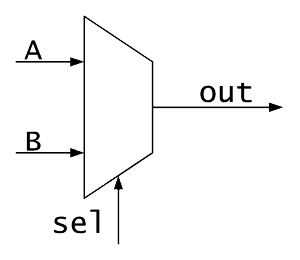
\includegraphics[width=0.30\linewidth]{Immagini/Multiplexer.png}
\caption{Esempio di un multiplexer a due ingressi.}
\end{figure}

\subsection{Demultiplexer}
Il contrario del multiplexer è il demultiplexer che accetta un segnale in serie e lo trasferisce in una delle possibili $n$ uscite a seconda dei $log(n)$ ingressi di selezione. 

\begin{figure}[!htb]
\centering
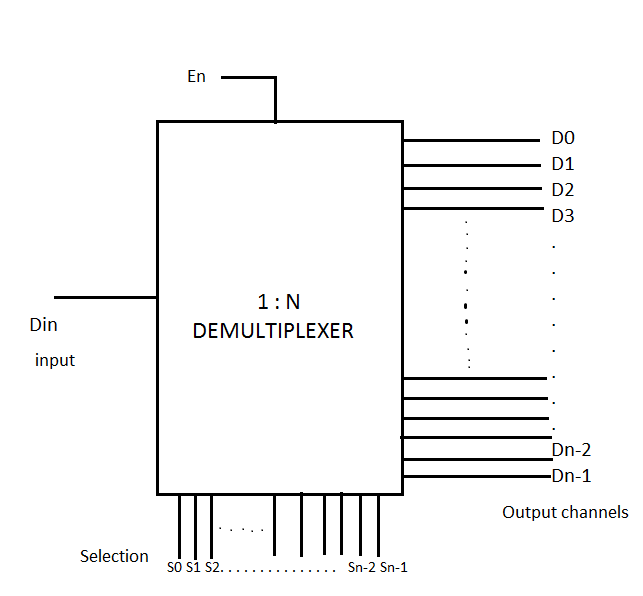
\includegraphics[width=0.50\linewidth]{Immagini/Demultiplexer.png}
\caption{Esempio di un demultiplexer a $n$ uscite e $log(n)$ ingressi.}
\end{figure}

\newpage
\subsection{Esercizio struttura calcolatore}
Rappresenta con una tabella di verità quattro istruzioni diverse:
\begin{enumerate}
    \item \textbf{mov AL, [64]:} (AL $\rightarrow$ [64]), che lavora sulla memoria
    \item \textbf{mov [64], AL:} ([64] $\rightarrow$ AL), che lavora sulla memoria
    \item \textbf{in AL, [64]:} ([64] $\rightarrow$ AL), che lavora su I/O
    \item \textbf{out [64], AL:} (AL $\rightarrow$ [64]), che lavora su I/O
\end{enumerate}
\begin{figure}[!htb]
\centering
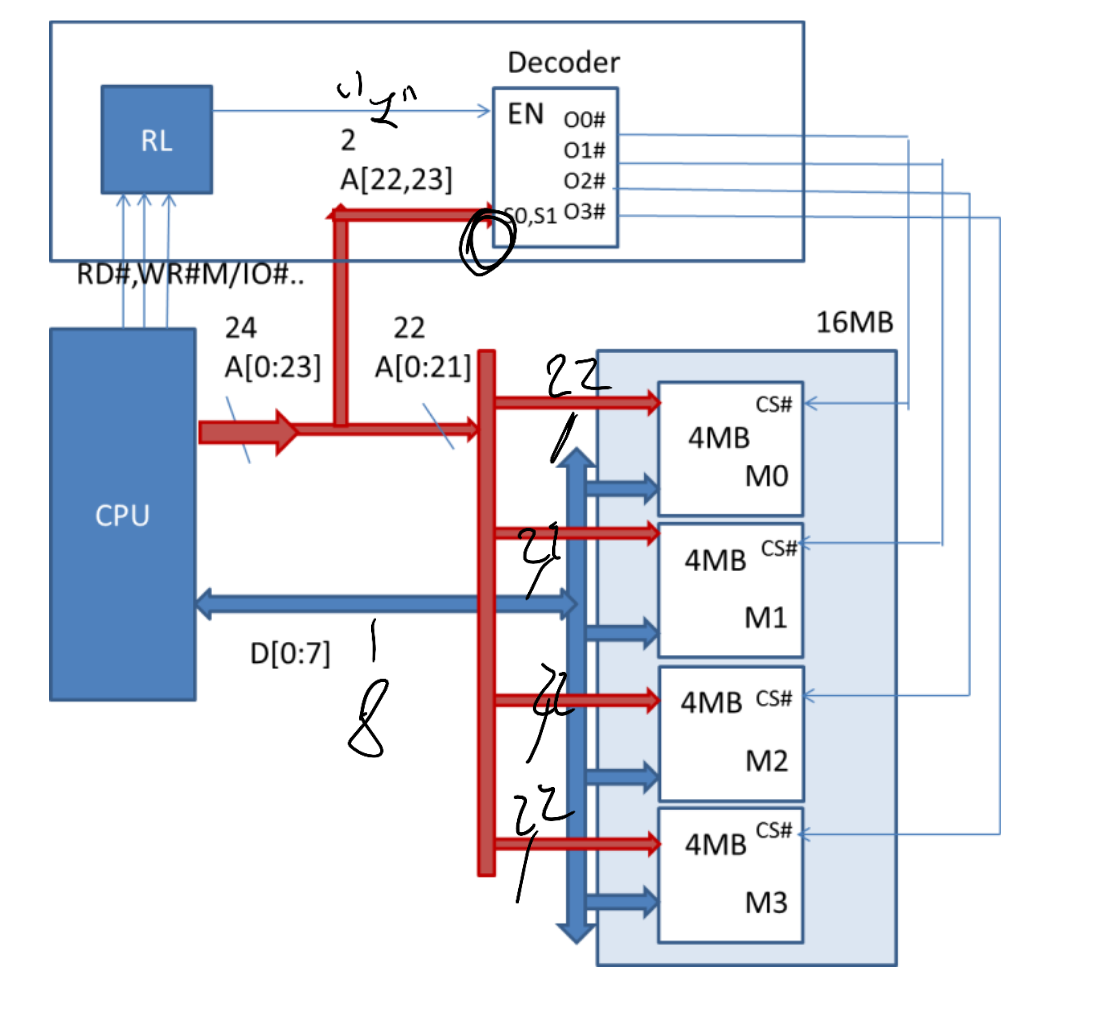
\includegraphics[width=0.60\linewidth]{Immagini/EsercizioBooleCalcolatore.png}
\caption{Esempio struttura di un calcolatore.}
\end{figure}

\textbf{\\Tabella di verità:}
\begin{center}
\begin{tabular}{|c |c c c | c c c c|} 
 \hline
 $\space$ & RD\# & RW\# & M-I/O\# & M-RD\# & M-WR\# & I/O-RD\# & I/O-WR\# \\
 \hline
 X & 0 & 0 & 0 & - & - & - & -  \\
 \hline 
 X & 0 & 0 & 1 & - & - & - & -  \\
 \hline
 2. & 0 & 1 & 0 & 1 & 0 & 0 & 0  \\
 \hline 
 3. & 0 & 1 & 1 & 0 & 0 & 1 & 0  \\
 \hline
 1. & 1 & 0 & 0 & 0 & 1 & 0 & 0  \\
 \hline 
 4. & 1 & 0 & 1 & 0 & 0 & 0 & 1  \\
 \hline
 * & 1 & 1 & 0 & 0 & 0 & 0 & 0  \\
 \hline 
 * & 1 & 1 & 1 & 0 & 0 & 0 & 0  \\
 \hline
\end{tabular}
\end{center}


\begin{itemize}
    \item Le prime due configurazioni sono vietate, perchè la CPU non potrà mai scrivere e leggere contemporaneamente.
    \item Le quattro configurazioni numerate sono le richieste dell'esercizio. 
    \item Le ultime due configurazioni sono possibili, per esempio nel caso in cui la CPU non debba fare nulla.
\end{itemize}

\newpage
\subsection{Reti sequenziali}
\hl{Reti logiche in cui in ogni istante le uscite dipendono non solo dalla
configurazione degli ingressi in quell’istante ma anche dalle configurazioni dagli ingressi negli istanti precedenti.} Devono, quindi, conservare memoria degli eventi passati nel proprio stato interno, dipendendo così anche dal tempo. Possono essere:
\begin{itemize}
    \item \textbf{Sincrone}, se le variazioni delle configurazioni di ingresso vengono sentite e modificano lo stato e le uscite in
    ogni istante.
    \item \textbf{Asincrone}, se le variazioni delle configurazioni di ingresso vengono sentite e modificano lo stato e le uscite solo
    in presenza di un opportuno evento di sincronizzazione.
\end{itemize}

\begin{figure}[!htb]
\centering
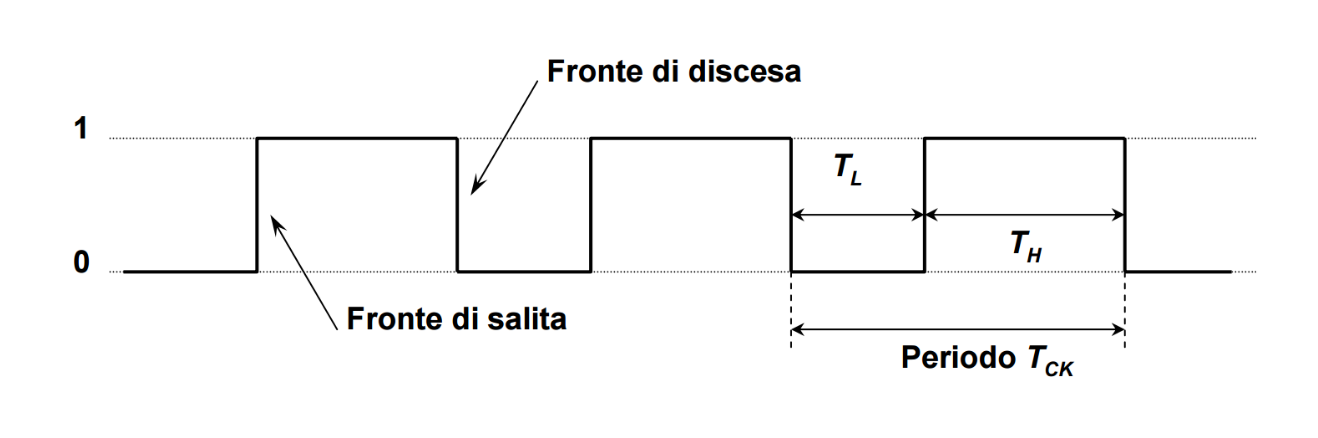
\includegraphics[width=0.80\linewidth]{Immagini/Clock.png}
\caption{Segnale di Clock.}
\end{figure}

\subsubsection{Alee}
\hl{Si dice \textbf{glitch} un impulso indesiderato dell’uscita in fase transitoria. Se una rete combinatoria può potenzialmente presentare un glitch allora si dice che è caratterizzata da un’\textbf{alea}.}
In alcuni casi le alee sono eliminabili con una sintesi opportuna, in altri casi non sono eliminabili. Le alee si classificano in:
\begin{itemize}
    \item \textbf{Alee statiche} se, in seguito ad un cambiamento di ingresso, l’uscita nel transitorio ha un cambiamento di valore
    mentre avrebbe dovuto rimanere costante.
    \item \textbf{Alee dinamiche} se, in seguito ad un cambiamento degli ingressi, l’uscita prima di cambiare valore definitivamente a regime, cambia più volte durante il transitorio.
\end{itemize}
\textbf{NB:} Le reti canoniche Sp e Ps evitano questo problema.

\hl{\\Si chiama \textbf{tempo di propagazione} il tempo impiegato dal gate a propagare in uscita il cambiamento del segnale di ingresso.}
\begin{figure}[!htb]
\centering
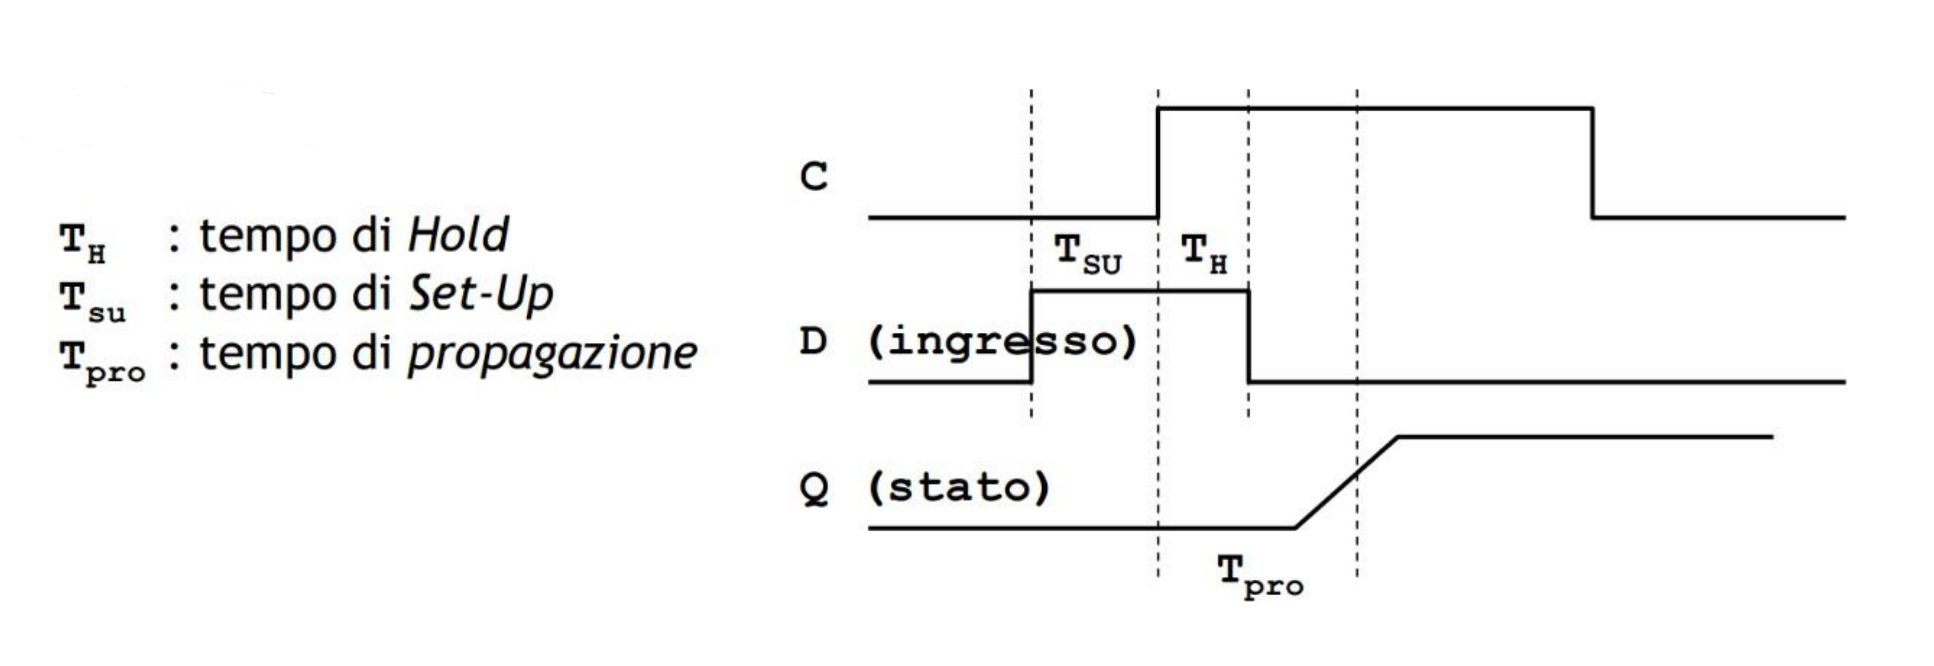
\includegraphics[width=1\linewidth]{Immagini/Tempi.png}
\caption{Tempo di Set-Up, Hold e Propagazione.}
\end{figure}

\newpage
\subsubsection{Elementi di Memeoria}
Gli elementi di base delle reti sequenziali sono gli elementi chiamati \textbf{bistabili}, capaci di mantenere al loro interno il valore 0 o il valore 1.

\subsubsection{Set Reset}
Il \textbf{Set Reset (SR)} è una rete con due ingressi S e R e una uscita Q (ed una uscita complementata Q\#) tale che l'uscita Q assume il valore 1 quando $S=1$ e $R=0$ e il valore 0 quando $S=0$ e $R=1$ e non cambi allorchè $S=R=0$.
La combinazione di ingresso $S=R=1$ non si verifica mai.

\begin{center}
\begin{tabular}{c | c || c | c} 
 S & R & Q & Q\# \\
 \hline
 0 & 0 & Q & Q\# \\
 0 & 1 & 0 & 1   \\
 1 & 0 & 1 & 0   \\
 1 & 1 & - & -   \\
\end{tabular}
\end{center}

\subsubsection{Latch e D-Latch}
\hl{Si definisce \textbf{Latch} un bistabile sincrono trasparente, capace di memorizzare o meno segnali di ingresso in funzione di un segnale di abilitazione.}
Il \textbf{D-Latch} è memoria capace di mantenere l’uscita se il segnale di clock non è attivo e di cambiare l’uscita campionando l’ingresso quando il clock è attivo.

\begin{center}
\begin{tabular}{c | c | c || c}
 C & S & R & Q\# \\
 \hline
 0 & - & - & Q \\
 1 & 0 & 0 & Q \\
 1 & 0 & 1 & 0 \\
 1 & 1 & 0 & 1 \\
 1 & 1 & 1 & - \\
\end{tabular}
\quad
\begin{tabular}{c | c || c | c}
 S & R & Q & Q\# \\
 \hline
 - & 0 & Q & Q\# \\
 0 & 1 & 0 & 1   \\
 1 & 1 & 1 & 0   \\
\end{tabular}
\end{center}

\subsubsection{Flip Flop}
\hl{Il \textbf{Flip Flop} è un dispositivo bistabile privo della proprietà di trasparenza.}
Nel flip flop il cambiamento della uscita non è conseguenza del cambiamento dell’ingresso di dato ma è conseguenza del cambiamento di un ingresso di controllo sincrono o asincrono.

\subsection{Registri}
I FF e i Latch D sono molto usati e se impiegati in parallelo (uno per ogni bit) possono registrale parole di n bit. Formano quindi i registri nella forma più semplice.

\subsubsection{Lettura}
Se il registro deve essere letto si deve selezinare quale dei registri va verso all’uscita. Nel register file ci sono due uscite possibili. L’uscita è selezionata dal multiplexer che contiene i numeri che corrispondenti ai due registri. Per la lettura l’abilitazione è immediata ma si collega ad un multiplexer che farà passare l’uscita solo della porta abilitata.

\subsubsection{Scrittura}
Un registro può essere sovrascritto con l’ingresso che arriva su writedata e con il write register che ne indica il numero e lo invia a un decoder che da uscita 1 a solo un registro, solo se c’è anche il segnale di Write che funge da “clock” o abilitatore alla scrittura.



\newpage
\section{ISA (Instruction Set Architecture)}
Il volcabolario delle istruzioni di un calcolatore è detto istruction set, possono essere diversi ma comunque sono simili fra loro. 
I più importanti sono il RISC-V, il MIPS e l'Intel x86.

\subsection{RISC-V Instruction Set}
Un’architettura aperta sviluppata dall’Università di
Berkeley a partire dal 2010 e ora gestito dalla RISC-V foundation.

\subsubsection{Operazioni aritmetiche}
Ci sono diverse operazioni:
\begin{itemize}
    \item \textbf{Somma aritmetica a tre operandi: \hl{add x5, x6, x7}.}
    \\Nel registro x5 viene messa la somma di x6 e x7.
    \item \textbf{Somma aritemtica immediata: \hl{addi x5, x6, 20}.}
    \\Nel registro x5 viene messa la somma di x5 e 20.
    \item \textbf{Sottrazione aritmetica a tre operandi: \hl{sub x5, x6, x7}.}
    \\Nel registro x5 viene messa la sottrazione di x6 e x7.
\end{itemize}

\subsubsection{Registri nel RISC-V}
Il RISC-V ha 32 registri da 32 bit:
\begin{itemize}
    \item \textbf{x0:} contiene il valore 0.
    \item \textbf{x1:} contiene l'indirizzo di ritorno.
    \item \textbf{x2:} puntatore allo stack.
    \item \textbf{x3:} puntatore globale.
    \item \textbf{x4:} puntatore al thread.
    \item \textbf{[x5-x7] e [x28-x31]:} contengono dati temporanei.
    \item \textbf{x8:} puntatore al frame
    \item \textbf{x9 e [x18-x27]:} contengono dati salvati 
    \item \textbf{x10 x11:} contengono gli argomenti o i valori di ritorno di una funzione.
    \item \textbf{[x12-x17]:} contengono gli argomenti delle funzioni.
\end{itemize}
\textbf{NB: Le operazioni aritmetiche usano operandi a registro.}

\begin{figure}[!htb]
\centering
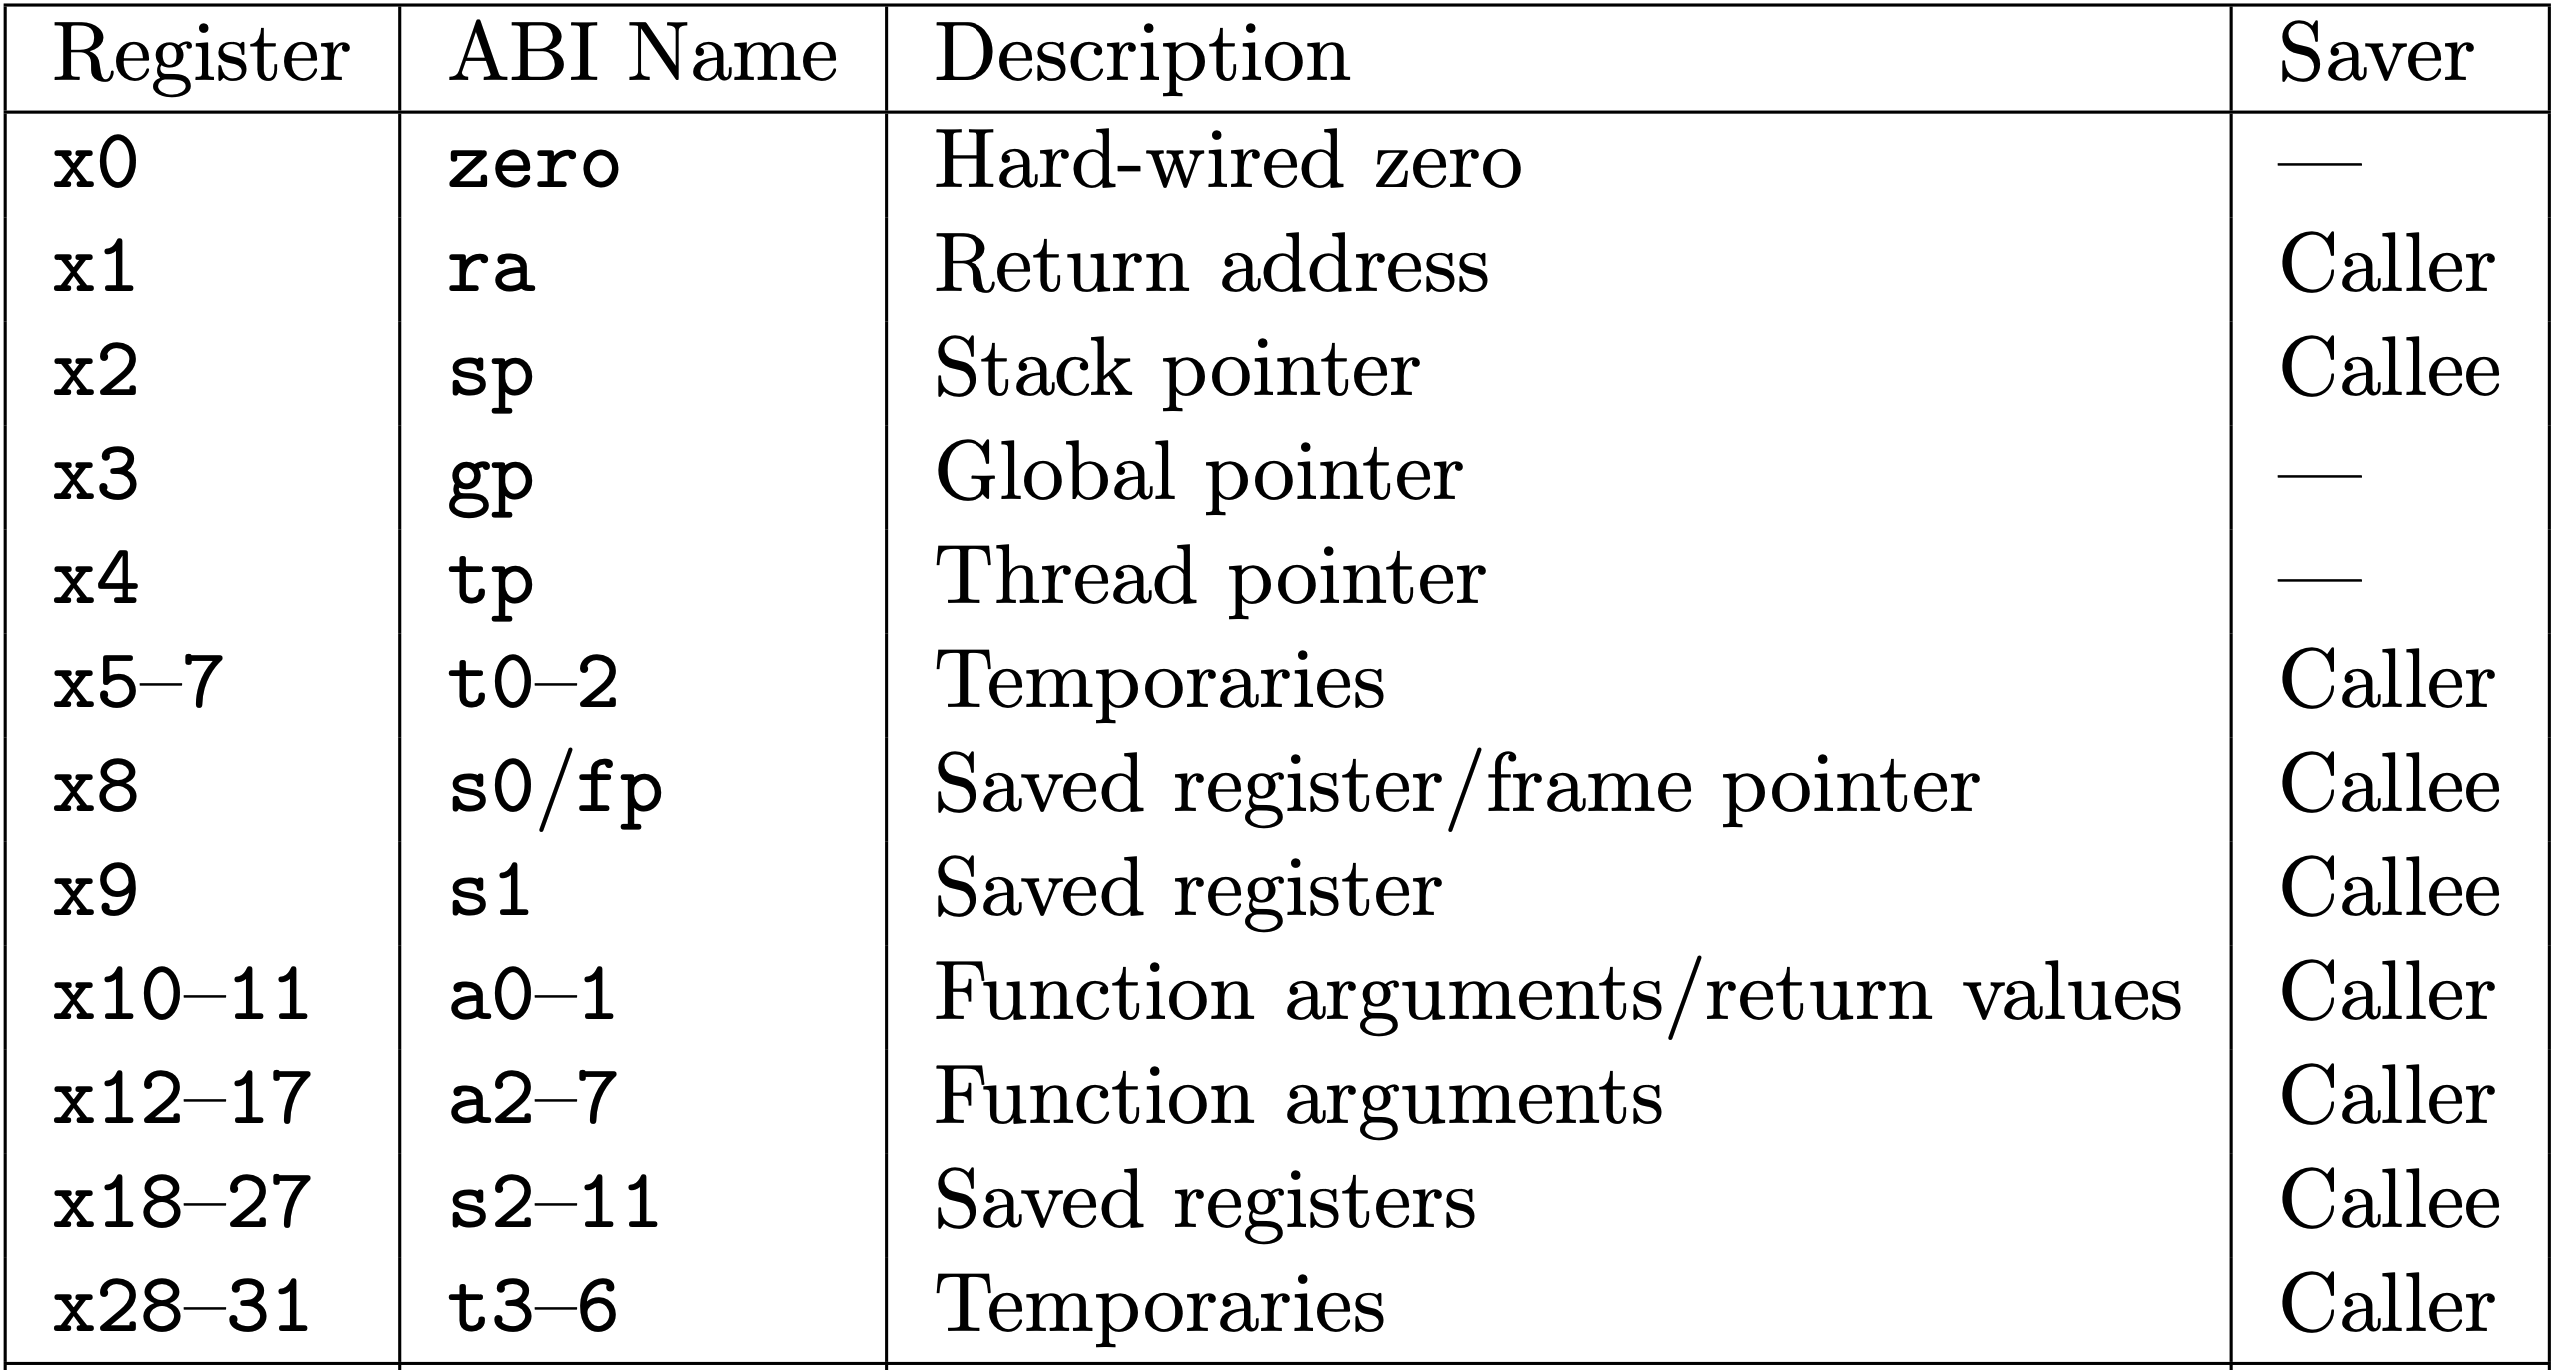
\includegraphics[width=0.70\linewidth]{Immagini/Registri.png}
\caption{Nomi registri standard RISC-V.}
\end{figure}


\newpage
\subsubsection{Codifica delle istruzioni}
Tutte le istruzioni RISC-V sono codificate come parole a 32-bit.
Nel caso delle istruzioni non immediate ti tipo R(registry) ha questa struttura:
\begin{center}
\begin{tabular}{|c|c|c|c|c|c|}
    \hline
    funct7 & rs2 & rs1 & funct3 & rd & opcode \\
    \hline
\end{tabular}
\end{center}
Dove: 
\begin{itemize}
    \item \textbf{funct7 e funct3} sono codici operativi aggiuntivi a 7 e 3 bit.
    \item \textbf{rs1 e rs2} sono i registri del primo e del secondo operando, i registri hanno sempre 5 bit.
    \item \textbf{rd} è il registro di destinazione, sempre 5 bit.
    \item \textbf{opcode} codice operativo dell'istruzione, che ha sempre 7 bit.
\end{itemize}
Nel caso delle istruzioni tipo I(immediate e load) la struttura è questa:
\begin{center}
\begin{tabular}{|c|c|c|c|c|}
    \hline
    immediate & rs1 & funct3 & rd & opcode \\
    \hline
\end{tabular}
\end{center}
Dove il campo immediate è il campo da 12 bit per il valore numerico passato.
Nelle istruzioni di tipo S(store) invece è questa:
\begin{center}
\begin{tabular}{|c|c|c|c|c|c|}
    \hline
    immediate & rs1 & rs2 & funct3 & immediate & opcode \\
    \hline
\end{tabular}
\end{center}
Dove il campo immediate è separato in due campi da 7 e 5 bit per avere i due registri sempre nella stessa posizione.

\subsubsection{Salti condizionati}
Sono due istruzioni per implementare processi decisionali, simili a un if seguito da go to. Ci sono diversi tipi di operazioni:
\begin{itemize}
    \item \textbf{Branch if equal, BEQ.}
    \item \textbf{Branch if not equal, BNE.}
    \item \textbf{Branch if lower than, BLT.}
    \item \textbf{Branch if greater of equal, BGE.}
    \item \textbf{Branch if less than unsigned, BLTU.}
    \item \textbf{Branch if greater or equal unsigned, BGEU.}
\end{itemize}

\subsubsection{Procedure}
Nelle procedure è necessario eseguire diverse operazioni, come il passaggio dei parametri, restituire un risultato, ecc... Nel RISC-V vengono usati diversi registri, dal x10 al x17 per il passaggio degli argomenti e del risultato e x1 per salvare l'indirizzo del chiamante.
Esistono alcune istruzioni per chiamare le procedure:
\begin{itemize}
    \item Istruzione per saltare all'inizio della procedura e salvare l'indirizzo del chiamante in x1: \textbf{jal x1, Procedura}
    \item Istruzione per ritornare al chiamante: \textbf{jalr x0, 0(x1)}
\end{itemize}

\subsubsection{Stack e Heap}
La struttura dati ideale per copiare il contenuto dei registri è lo \textbf{stack}, una coda di tipo LIFO. In RISC-V il puntatore allo stack è il registro x2 (o sp). Lo stack pointer viene incrementato o decrementato di una parola ogni volta che si toglie o si inserisce il contenuto di un registro.
Alcuni programmi RISC-V usano il frame pointer (fp, registro x8) per puntare alla prima parola del frame di una procedura, per convenienza rispetto allo sp che invece potrebbe cambiare allocando vettori e strutture locali.
Lo stack parte dalla parte alta degli indirizzi della memoria e si espande verso il basso, l'\textbf{heap}, l'area riservata agli elementi dinamici si muove al contrario.

\newpage
\section{Archittetura della CPU}
\begin{figure}[!htb]
\centering
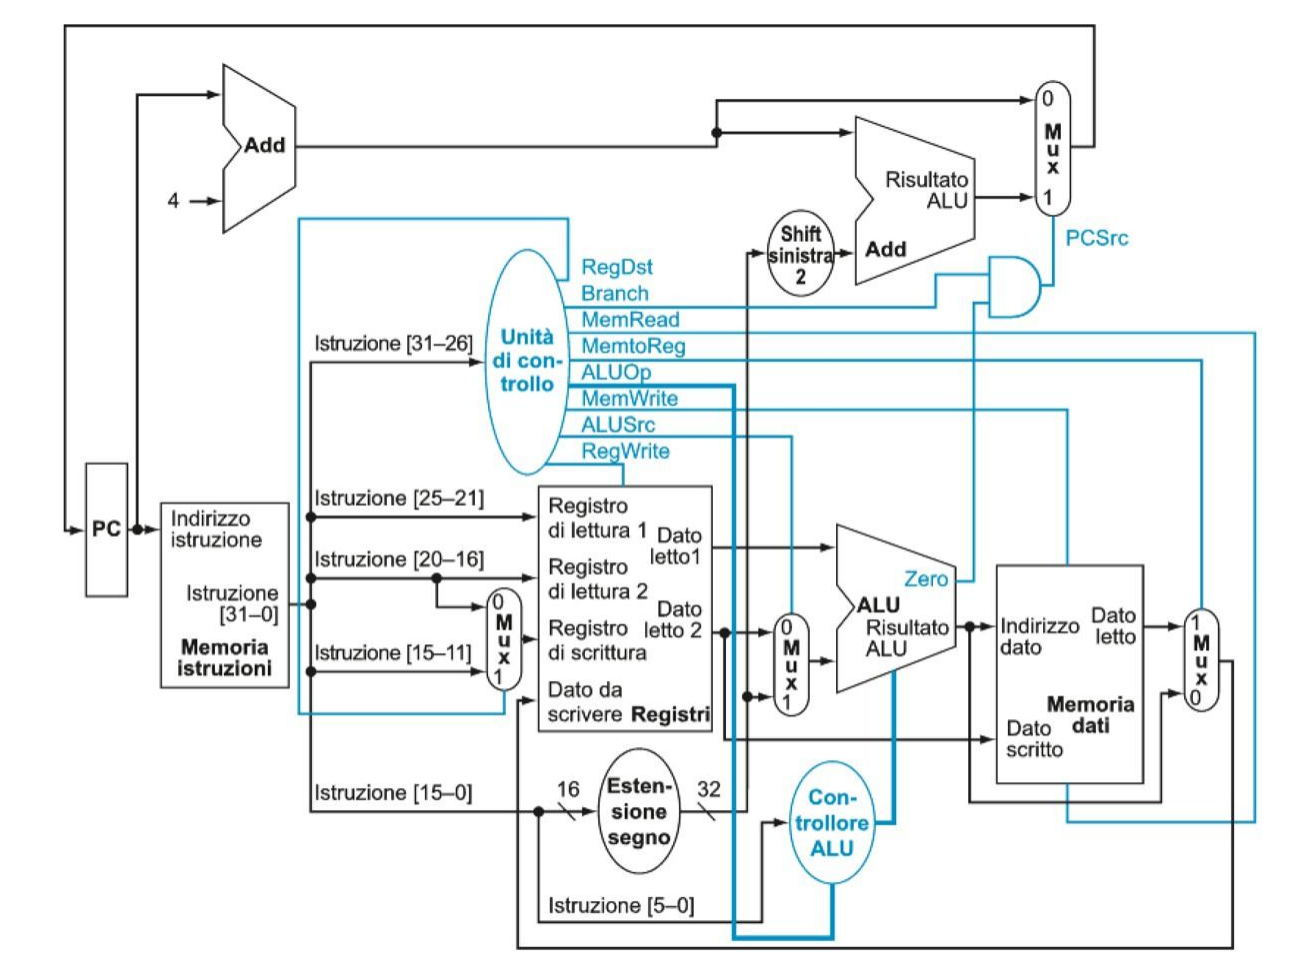
\includegraphics[width=0.85\linewidth]{Immagini/CpuRISC-V.png}
\caption{Archittetura semplice e monocilco di una CPU Risc-V.}
\end{figure}

L'esecuzione di un istruzione si divide in 5 fasi:
\begin{itemize}
    \item \textbf{Fetch:} si occupa di prendere l'istruzione tramite il suo indirizzo nel program counter (PC).
    \item \textbf{Decode:} si occupa di tradurre l'istruzione, dividendo i bit per la fase di execute.
    \item \textbf{Execute:} si occupa di eseguire le varie operazioni, in questa fase i calcoli sono destinati all'alu.
    \item \textbf{Memory:} per alcune istruzioni è necessario attivare la memoria.
    \item \textbf{Write Back:} si occupa di riscrivere il risultato.
\end{itemize}
L'unità di controllo si occupa di gestire i vari segnali, tra cui:
\begin{itemize}
    \item \textbf{RegWrite:} per scrivere sui registri al termine di un’operazione di ALU o di lettura.
    \item \textbf{MemWrite e MemRead:} per leggere o scrivere i dati sulla memoria di dato.
    \item \textbf{AluOp:} è l’insieme dei segnali di controllo che indicano all’ALU l’operazione da fare.
    \item \textbf{Zero:}  il segnale che esce dal PSW della ALU per indicare se c’è stata una condizione di zero.
    \item \textbf{Branch:} segnale che indica se c'è stato un branch.
    \item \textbf{MemToReg:} segnale inviato a un multiplexer che serve per scrivere un dato dalla memoria a un registro.
    \item \textbf{AluSrc:} segnale inviato al multiplexer che si occupa di mandare all'alu il valore di un registro o il valore immediato nell'istruzione.
    \item \textbf{PsScr:} risultato dell'AND fra il segnale zero e il segnale branch, se uguale a uno imposta il pc all'indirizzo del salta.
\end{itemize}
Altri componenti importanti sono l'estensione del segno da 16 bit a 32 bit e lo shift a sinistra di 2.

\subsection{Alee}
Esistono molte situazioni in cui la pipeline non è ideale. La pipeline ideale però può nella realtà avere difficoltà nella esecuzione a causa di diversi problemi chiamati alee, con tre tipi di conflitti:
\begin{itemize}
    \item \textbf{Alee strutturali}
    \item \textbf{Alee di dato}
    \item \textbf{Alee di controllo}
\end{itemize}

\subsubsection{Alee strutturali}
\subsubsection{Alee di dato}
\subsubsection{Alee di controllo}


\newpage
\section{Memorie}
\hl{La memoria è l’ unità logica di memorizzazione di dati nel calcolatore.} Nell’architettura dei calcolatori si distingue la memoria centrale, in diretto collegamento con la CPU e che contiene l’informazione in uso, dalla memoria di massa che ha il compito come periferica di I/O di mantenere dati ed istruzioni in modo permanente.
Esistono diversi tipi di dispositivi di memoria che possono essere classificati in base a:
\begin{itemize}
    \item Capacità.
    \item Caratteristiche fisiche.
    \item Modalità di accesso.
    \item Organizzazione.
    \item Prestazioni.
\end{itemize}

\subsection{Capacità}
La capacità è calcolata come: 
\[ C = M \times N\]
Dove N è la grandezza della parola e M è il numero di parole.

\subsection{Caratteristiche fisiche}
Le memorie possono essere classificate in base alle caratteristiche fisiche:
\begin{itemize}
    \item Memorie a semiconduttore.
    \item Memorie a superficie magnetica.
    \item Memorie ottiche.
\end{itemize}
Le memorie centrali sono realizzate con tipologia a semiconduttore; la memoria di massa, quale i dischi, a superficie magnetica o di tipo ottico (come i CD) e sempre di più anche a semiconduttore (memorie a stato solido). 
Possono essere categorizzate anche in base al consumo, all'affidabilità e in base alla durevolezza. In base alla durevolezza o volatilità, si possono definire due categorie:
\begin{itemize}
    \item Memorie che perdono le informazioni se non alimentate elettricamente, come le RAM.
    \item Memorie che mantengono le informazioni anche se non alimentate elettricamente, come l’hard disk o le flash.
\end{itemize}
Le memorie volatili sono molto utilizzate, anzi costituiscono la massima parte della memoria centrale in quanto hanno tempi di accesso ossia latenza molto inferiori a quelli di altre memorie. Tra le memorie volatili ne esistono diverse categorie:
\begin{itemize}
    \item \textbf{Memorie statiche:} costituite da bistabili sincroni o a sincroni che mantengono il bit memorizzato fino ad una nuova riscrittura con FF o D-Latch.
    \item \textbf{Memorie dinamiche:} il bit è memorizzato sotto forma di carica all’interno di un condensatore, a causa delle correnti di scarica e il valore 1 memorizzato diventa 0. È quindi necessario che periodicamente si provveda a leggere ogni bit e a riscrivere i bit con valore 1.
\end{itemize}

\subsection{Modalità di accesso}
L’architettura della memoria definisce la sua modalità di accesso. A seconda della modalità di accesso si hanno diverse prestazioni e diversi tempi di accesso:
\begin{itemize}
    \item \textbf{Accesso sequenziale:} se per accedere ad un dato in una fissata posizione della memoria è necessario accedere a tutti i dati memorizzati in posizioni precedenti.
    \item \textbf{Accesso diretto:} se è possibile avere un accesso direttamente alla locazione di memoria voluta senza dovere accedere alle locazioni precedenti.
    \item \textbf{Accesso casuale:} è un accesso diretto in cui il tempo di accesso è costante e non dipende nè dall’indirizzo nè dalla precedente locazione acceduta.
    \item \textbf{Accesso associativo:} e per accedere ad un dato bisogna cercare un’associazione tra l’indirizzo e il contenuto. 
\end{itemize}

\subsubsection{Memorie RAM}
Le memorie RAM (Random access memory) sono memorie volatili a lettura e scrittura in cui il tempo di accesso è costante per ogni locazione di memoria indirizzata. Perciò hanno per definizione modalità di accesso casuale. Ci sono due categorie: 
\begin{itemize}
    \item \textbf{SRAM (Static RAM)}.
    \item \textbf{DRAM (Dynamic RAM)}.
\end{itemize}

\subsubsection{Memorie ROM}
Le memorie ROM (Read only memory) sono memorie di sola lettura, esse non hanno logica dedicate per la scrittura ma vengono scritte attraverso differenti apparati tecnologici:
\begin{itemize}
    \item \textbf{PROM (Programmable ROM:} programmabili una sola volta impiegando un pin speciale.
    \item  \textbf{EPROM (Eraseable programmable ROM):} PROM ma cancellabili in toto con luce ultravioletta.
    \item  \textbf{EEPROM (Electrically eraseable programmable ROM):} PROM che sono cancellabili elettricamente senza doverle estrarre dalla scheda.
    \item \textbf{FLASH:}  sono un tipo speciale di EEPROM leggibili e scrivibili a blocchi senza estrarle dal circuito.
\end{itemize}

\subsection{Organizzazione della memoria}
La memoria vista fino ad ora e’ una tipica architettura non gerarchica dove tutte le memorie sono uguali dal punto di vista logico nello spazio di indirizzamento. Chi progetta il calcolatore vede tutti i dispositivi di memoria centrale nello stesso modo anche se hanno tipologie diverse.

\subsubsection{Organizzazione gerarchica}
Il calcolatore contiene memorie di tipi, prestazioni e costi
diverse. La gerarchia e’ fatta in modo tale da avere ai livelli piu’ alti memorie piu’ piccole e veloci, ma con un meccanismo di accesso che ottimizza l’uso di tutte le memorie. 
Questo è possibile grazie a due prorpietà: 
\begin{itemize}
    \item \textbf{Localita spaziale:} è la proprietà dei programmi per cui accedendo ad un dato è assai probabile che si debba accedere ad un dato allocato in uno spazio in memoria localmente vicino.
    \item \textbf{Località temporale:} è la proprietà dei programmi per cui accedendo ad un dato è assai probabile che si debba accedere nuovamente ad esso in un breve intervallo di tempo.
\end{itemize}
I programmi non vedono la gerarchia ma referenziano i dati come se fossero sempre in memoria centrale, perciò bisogna mantenere il più vicino possibile alla CPU dati utilizzati più recentemente.

\begin{figure}[!htb]
\centering
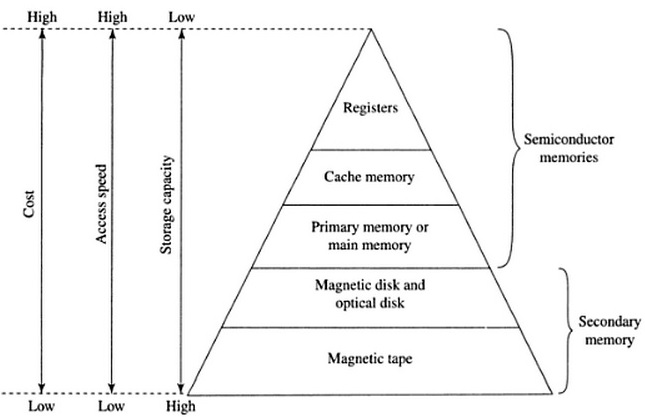
\includegraphics[width=0.60\linewidth]{Immagini/MemoryHierarchy.jpg}
\caption{Piramide della grarchia delle memorie.}
\end{figure}

\subsubsection{Memorie Cache}
\hl{La cache è una memoria centrale veloce, volatile e ad accesso associativo. Le memorie cache sono realizzate normalmente con tecnologia SRAM.}

\begin{figure}[!htb]
\centering
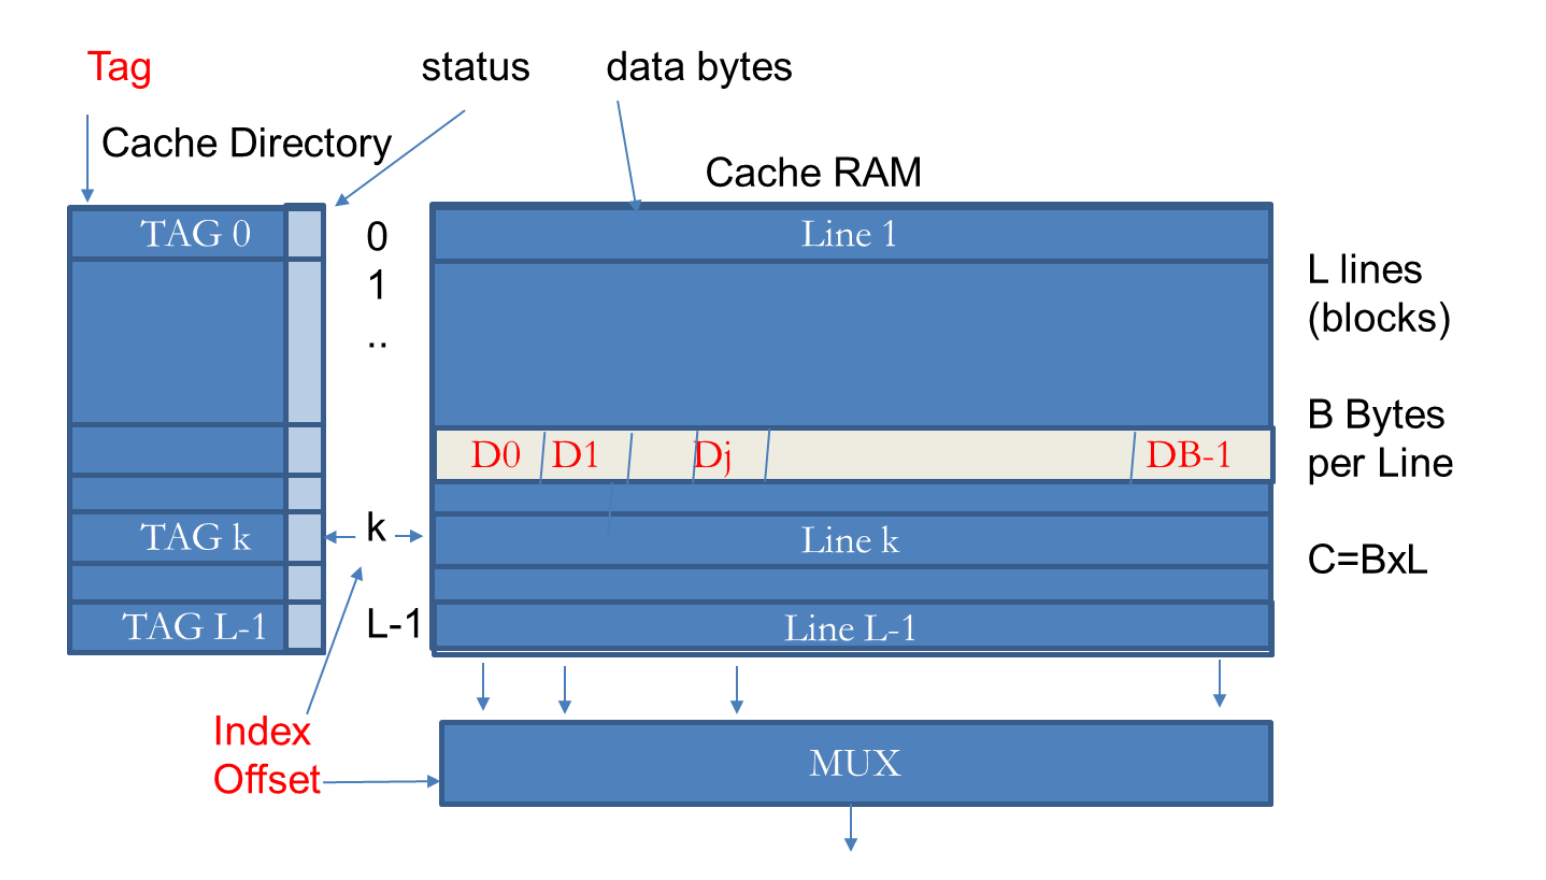
\includegraphics[width=0.80\linewidth]{Immagini/CacheGenerale.png}
\caption{Descrizione grafica cache.}
\end{figure}

Nello specifico:
\begin{itemize}
    \item La cache RAM contiene L blocchi di dati o linee, ogni linea contiene B byte. La capacità è quindi C = L $\times$ B.
    \item Può essere calcolato un offset nell'indirizzo partendo da B, nello specifico l'offset è $log_2(B)$.
    \item L'offset serve a il multiplexer per controllare se c'è stata una hit.
    \item Essendo un accesso associativo, non è detto che il dato si trovi in cache. Esiste perciò una parte della cache detta anche cache directory che contiene i tag ed eventuali bit di stato.
    \item I bit di tag sono tutti quelli rimanenti tolto l'offset, quindi $\text{tag} = \text{na} - log_2(B)$. Dove na è il numero di bit dell'indirizzo.
\end{itemize}
La cache può essere classificata a seconda del grado di associatività per quel che riguarda il piazzamento dei dati, in tre categorie:
\begin{itemize}
    \item \textbf{Cache fully associative:} è la cache descritta precedentemente con piazzamento completamente associativo ossia senza vincoli sull’indice in cui la linea può essere piazzata.
    L’indirizzo è quindi composto da una parte di offset e una parte di Tag che vengono usati per essere associati a tutte le linee della cache. Questa architettura è la più efficiente, ha mediamente la miss rate più bassa ma è anche la più costosa per il costo della logica di controllo dei tag. È inoltre la più costosa anche per decidere la politica di rimpiazzamento nel caso di cache piena.
    
    \item \textbf{Cache direct mapped:} la cache direct mapped prevede una sola possibilità di piazzamento per ogni linea . Ogni linea infatti usa una parte del tag come chiave unica di indice. Ogni linea se è presente sulla cache può risiedere in una sola posizione data
    dalla parte di indirizzo chiamata index. La parte di index è la parte meno significativa del tag. In questo modo due blocchi adiacenti vengono mappati in due linee consecutive e non si sovrappongono. L’indirizzo è quindi composto da una parte di offset, da una parte di index di $\text{Ni} = log_2(L)$, restanti sono i bit di Tag che vengono usati per essere associati al tag memorizzato all’interno. È la cache potenzialmente con il più alto miss rate ma è anche la
    meno costosa. Di fatto l’index fa da indirizzo per indirizzare solo quella linea sia della cache directory che della cache ram che puo’ contenere il dato.
    \begin{figure}[!htb]
    \centering
    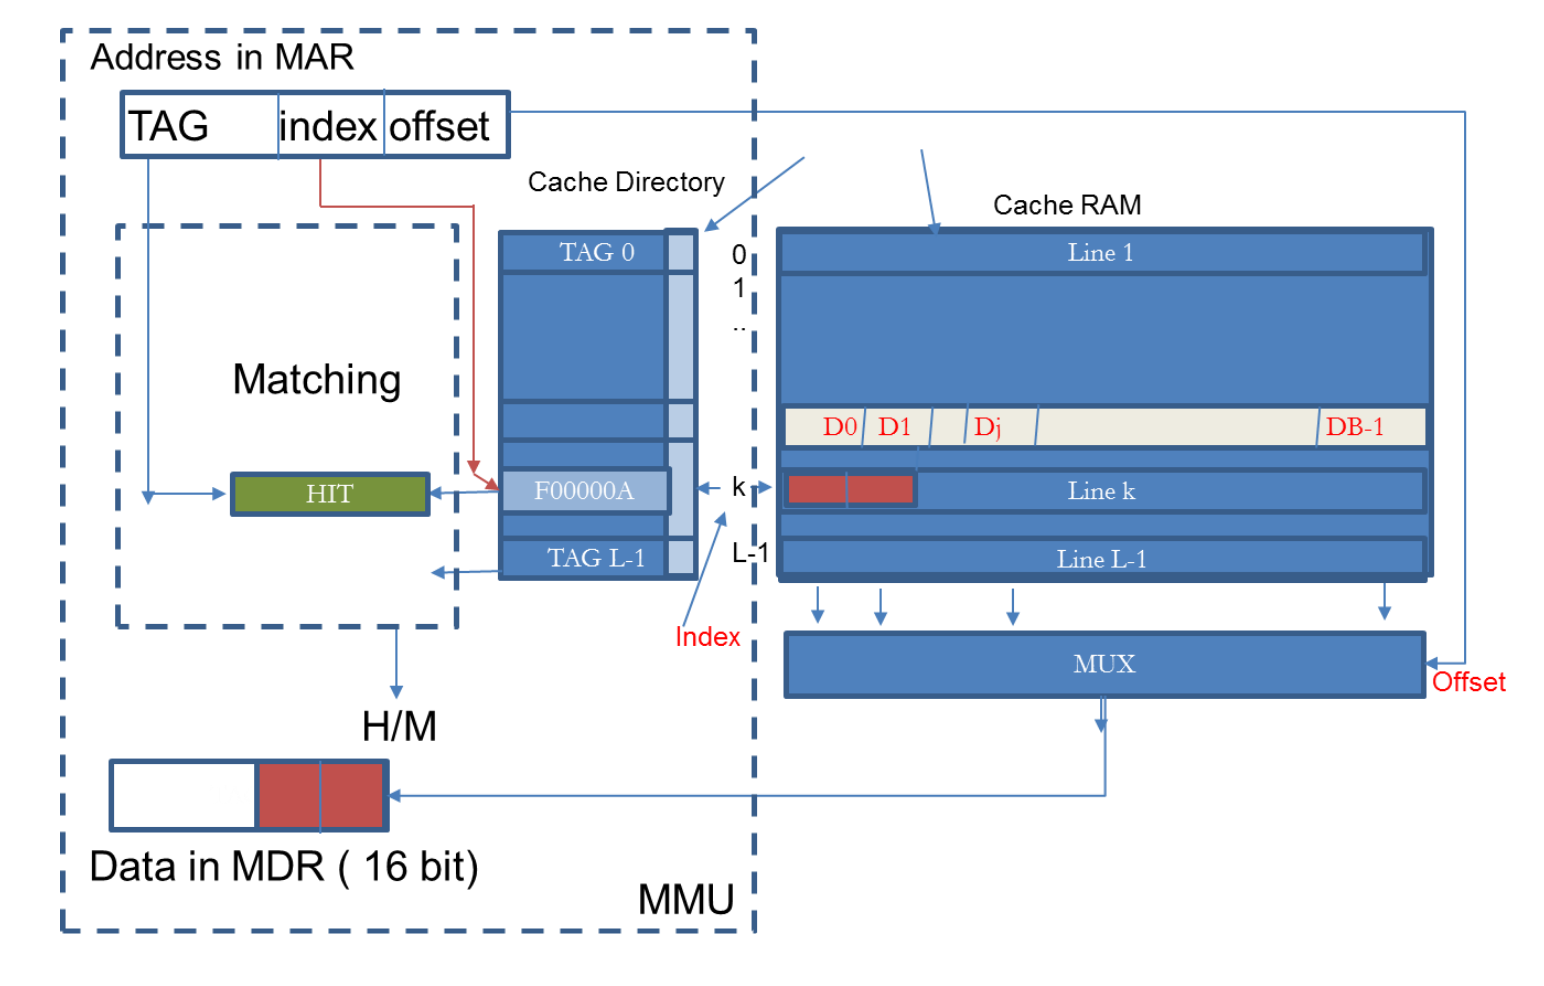
\includegraphics[width=0.80\linewidth]{Immagini/CacheDirectMapped.png}
    \caption{Descrizione grafica cache.}
    \end{figure}
    
    \newpage\item \textbf{Cache n-way associative} è la cache più usata, compromesso tra le architetture precedenti. Le linee della cache sono divise in S set da n vie ognuna. Ogni linea del livello inferiore della gerarchia può essere piazzata in un solo set ma in una qualsiasi delle n linee dentro al set. È una cache quindi direct mapped a livello di set ma totalmente associativa dentro al set. Il miss rate è minore rispetto al caso precedente perchè ci sono più possibilità di mantenere la linea nella cache senza doverla  rimpiazzare. L’indirizzo è composto da una parte di offset, da una parte di index di $\text{Ni}= log_2(S)$ dove $S=\frac{L}{n}$ è il numero di set e i restanti bit di Tag che vengono usati per essere associati al tag memorizzato all’interno.
    \begin{figure}[!htb]
    \centering
    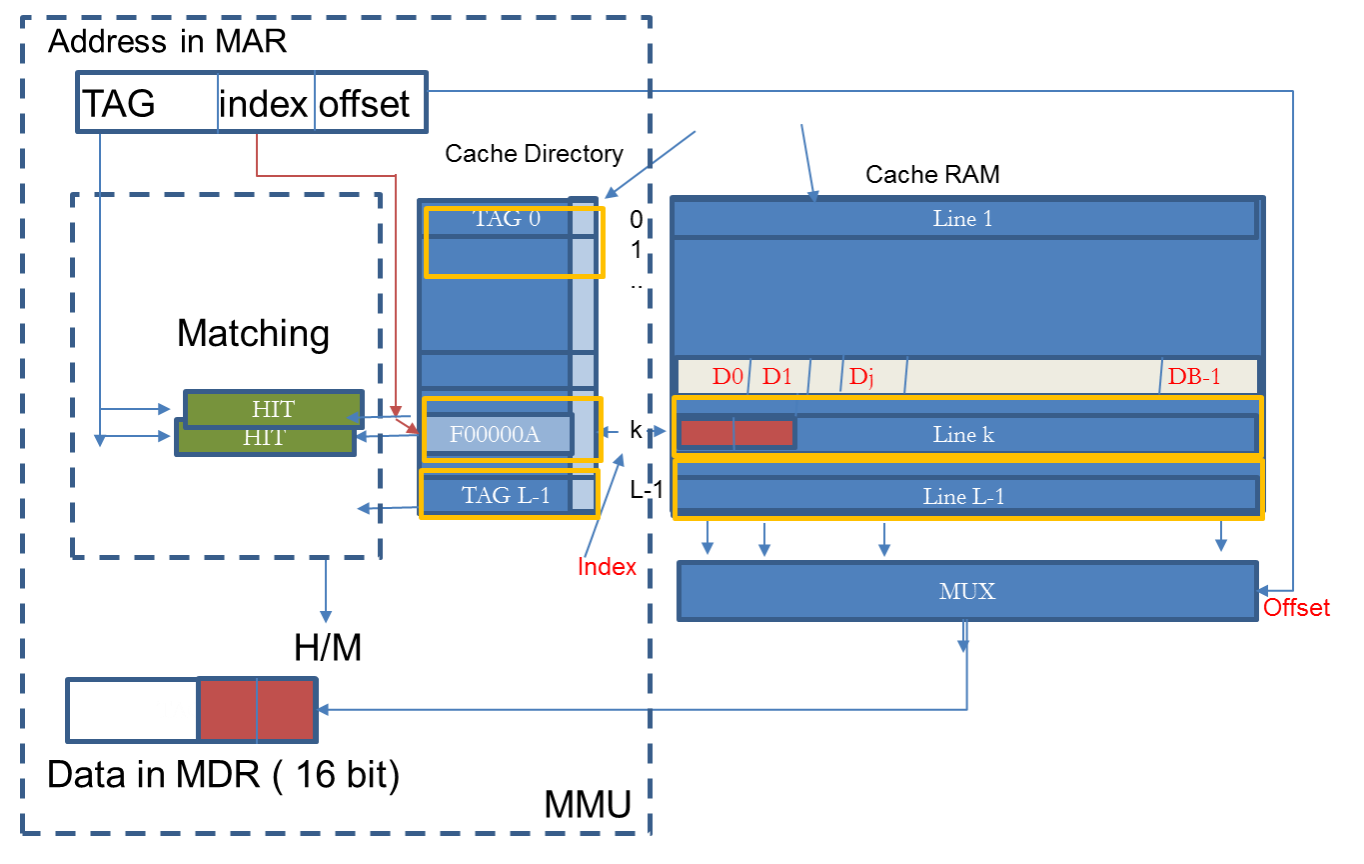
\includegraphics[width=0.80\linewidth]{Immagini/Cachenway.png}
    \caption{Descrizione grafica cache n-way associative.}
    \end{figure}
\end{itemize}

\subsubsection{Prestazioni nell'organizazzione gerarchica}
Le prestazioni delle memorie si misurano in tempo, la latenza per le memorie si chiama tempo di accesso mentre il throughput si calcola come reciproco del tempo di ciclo.
Nello speicifico:
\begin{itemize}
    \item \textbf{Blocco:} unità di informazione minima scambiata fra livelli.
    \item \textbf{Hit:} un accesso alla memoria che trova l'informazione cercata nel livello superiore.
    \item \textbf{Hit rate:}  frequenza di accessi trovati nel livello superiore (h).
    \item \textbf{Miss rate:} 1-h.
    \item \textbf{Hit time:} tempo di accesso al livello superiore $T_h$.
    \item \textbf{Miss penalty:} tempo per rimpiazzare un blocco nel livello superiore più il tempo per fornirlo alla CPU. Quindi $T_{mp} = T_h + T_{miss}$.
\end{itemize}
Il tempo di accesso può essere calcolato come:
\[
    T_{acc} = h T_h + (1-h)T_{mp} = T_h + (1-h)T_{miss}
\]

\subsection{Miss}
Ci sono tre tipologie di miss diverse:
\begin{itemize}
    \item \textbf{Compulsory (obbligatorie)} se sono inevitabili, esse si verificano quando la linea richiesta non è mai stata in cache.
    \item \textbf{Conflict} se sono dovute a un conflitto dovute alla limitata associatività, ovvero, il dato viene richiesto nella cache, sarebbe stato presente ma è stato rimpiazzato perché un'altra linea con lo stesso index è stata richiesta in seguito e a causa della limitataa ssociatività ha preso il suo posto.
    \item \textbf{Capacity} se sono dovute alla limitata capacità della cache, ovvero, la linea sarebbe stata presente ma essendo la cache di capacità limitata essa è stata rimpiazzata da un’altra.
\end{itemize}
\subsubsection{Esercizio:}
Si deve eseguire un programma con un ciclo di 10 iterazioni.
In ogni ciclo si devono leggere le variabili var1,var2,var3 e var4 che sono allocate in memoria agli indirizzi rispettivamente F000A023, F000A021, A000A022, F000A025.
\begin{enumerate}
    \item Con uno spazio di indirizzamento a 32 bit ed una cache direct mapped con linee di 16B di dati e di capacità di 1Mbyte, quante miss e di che tipo si verificano?
    \item E se la cache è a 2 vie associative?
    \item E se la cache è come nel primo caso ma con 32 B di dimensione di Linea?
    \item E se è come il secondo e terzo caso insieme?
\end{enumerate}
Nel caso 1. si ha che la cache ha 256k righe, quindi ci sono ha 10 bit di tag, 18 bit di indice e 4 bit di offset.

\begin{figure}[!htb]
\centering
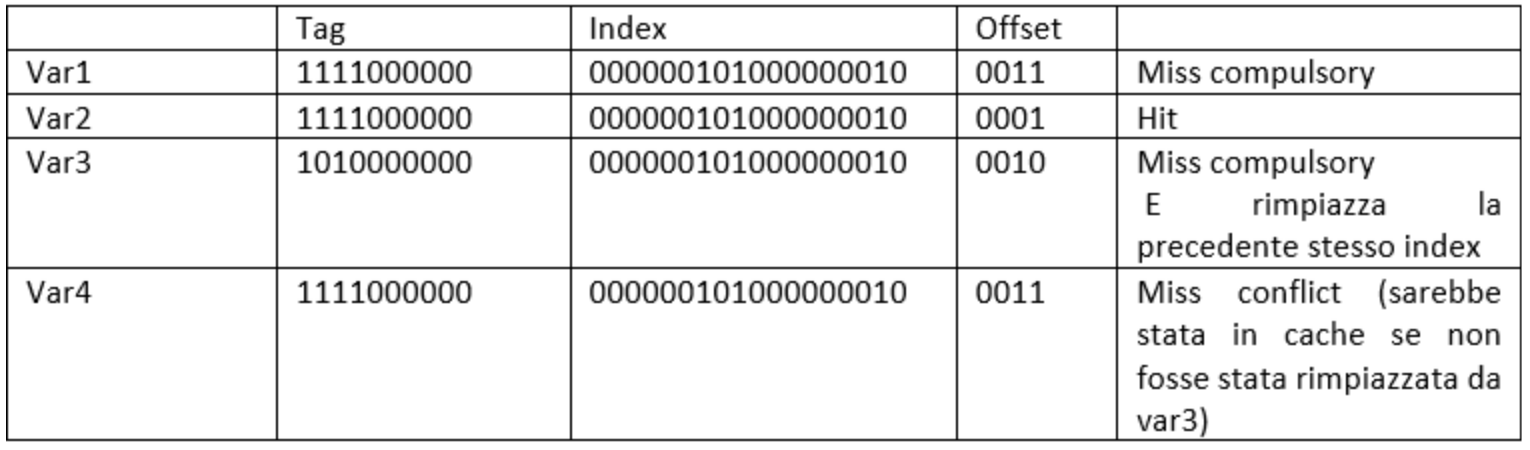
\includegraphics[width=0.80\linewidth]{Immagini/EsercizioCache.png}
\caption{Descrizione grafica cache.}
\end{figure}

Le quattro variabili hanno lo stesso indix ma tag diverso, quindi, nella prima iterazione: 
\begin{itemize}
    \item Var1 ha un miss compulsory, perchè la cache è vuota.
    \item Var2 ha un hit, perchè avendo lo stesso tag di var1 sono state caricate pure var2 e var4.
    \item Var3 ha un miss compulsory, perchè non è presente nella cache e quindi viene pure caricata.
    \item Var4 ha un miss conflict, perchè era stato caricata ma poi è stat sostituita da var3, però viene caricata in cache.
\end{itemize}
In tutte le altre interazioni le prime due variabili fanno una hit, dato che var4 al fine di ogni iterazione viene caricato, invece var3 e var 4 ha in miss conflict, perchè si sostituiscono a vicenda.

\subsection{Scrittura}
Avendo più livelli di memorie cache ci sono diverse strategie per scrivere i dati:
\begin{itemize}
    \item \textbf{write-back:} è la strategia per cui la scrittura avviene solo al livello più alto della gerarchia e viene copiato nei livelli più bassi solo se la linea viene rimpiazzata o al termine della esecuzione del task . È il metodo più efficiente dal punto di vista del tempo di accesso.
    \item \textbf{write through:} è la strategia per cui ad ogni scrittura il dato viene scritto in tutti i livelli della gerarchia.
\end{itemize}

\subsection{Memoria virtuale}
\hl{Memoria virtuale è il nome che viene dato al livello della gerarchia delle memorie che si occupa del trasferimento dei dati tra la memoria principale e il disco.} \\La memoria virtuale permette ai singoli programmi di espandere il proprio spazio di indirizzamento oltre i limiti
della memoria principale. Caratteristica ancora più importante è il fatto che la memoria virtuale supporta la condivisione della memoria
principale tra più processi attivi simultaneamente, in modo protetto.
La memoria viene divisa in blocchi (chiamate PAGINE) ognuna con propri bit di stato, tra cui quelli P di protezione per indicare che solo alcuni owner possono averne l’accesso.\\
Il meccanismo della memoria virtuale vede la memoria centrale come una cache della memoria di massa, dove i blocchi sono le pagine. La memoria centrale è fully associative e il meccanismo di rimpiazzamento è LRU.

\begin{figure}[!htb]
\centering
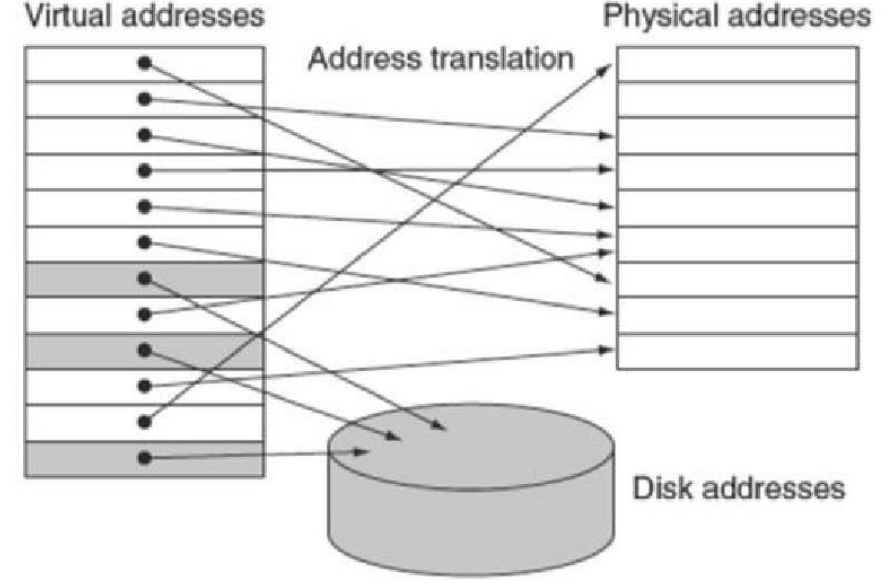
\includegraphics[width=0.50\linewidth]{Immagini/MemoriaVirtuale.png}
\caption{Descrizione grafica memoria virtuale.}
\end{figure}

La parte alta non funziona come tag con un accesso associativo ma viene usato come indice in un processo che è chiamato address translation ed avviene attraverso una tabella (page table).

\subsubsection{Page fault}
Il page fault richiede l’accesso alla memoria di massa che può essere 100 000 volte più lento e il processo di gestione è fatto in software non in hardware con milioni di cicli di clock, così si possono usare algoritmi
intelligenti per la allocazione.
La memoria è completamente associativa per avere il minor numero di miss ossia di page fault. La tecnica di scrittura è sempre write-back, il write through sarebbe troppo costoso. La pagina è a sua volta in memoria, ad un indirizzo indicato in un registro specifico, ossia il PTR Page table register.

\newpage
\subsubsection{Address mapping}
In base alla traduzione dell’indirizzo, alcune pagine si trovano effettivamente in memoria centrale, ossia in memoria fisica e la
traduzione trasforma il virtual page number in un physical page number.
Il primo accesso si ottiene la rilocazione dell’indirizzo virtuale in fisico e l’allocazione di memoria.

\begin{figure}[!htb]
\centering
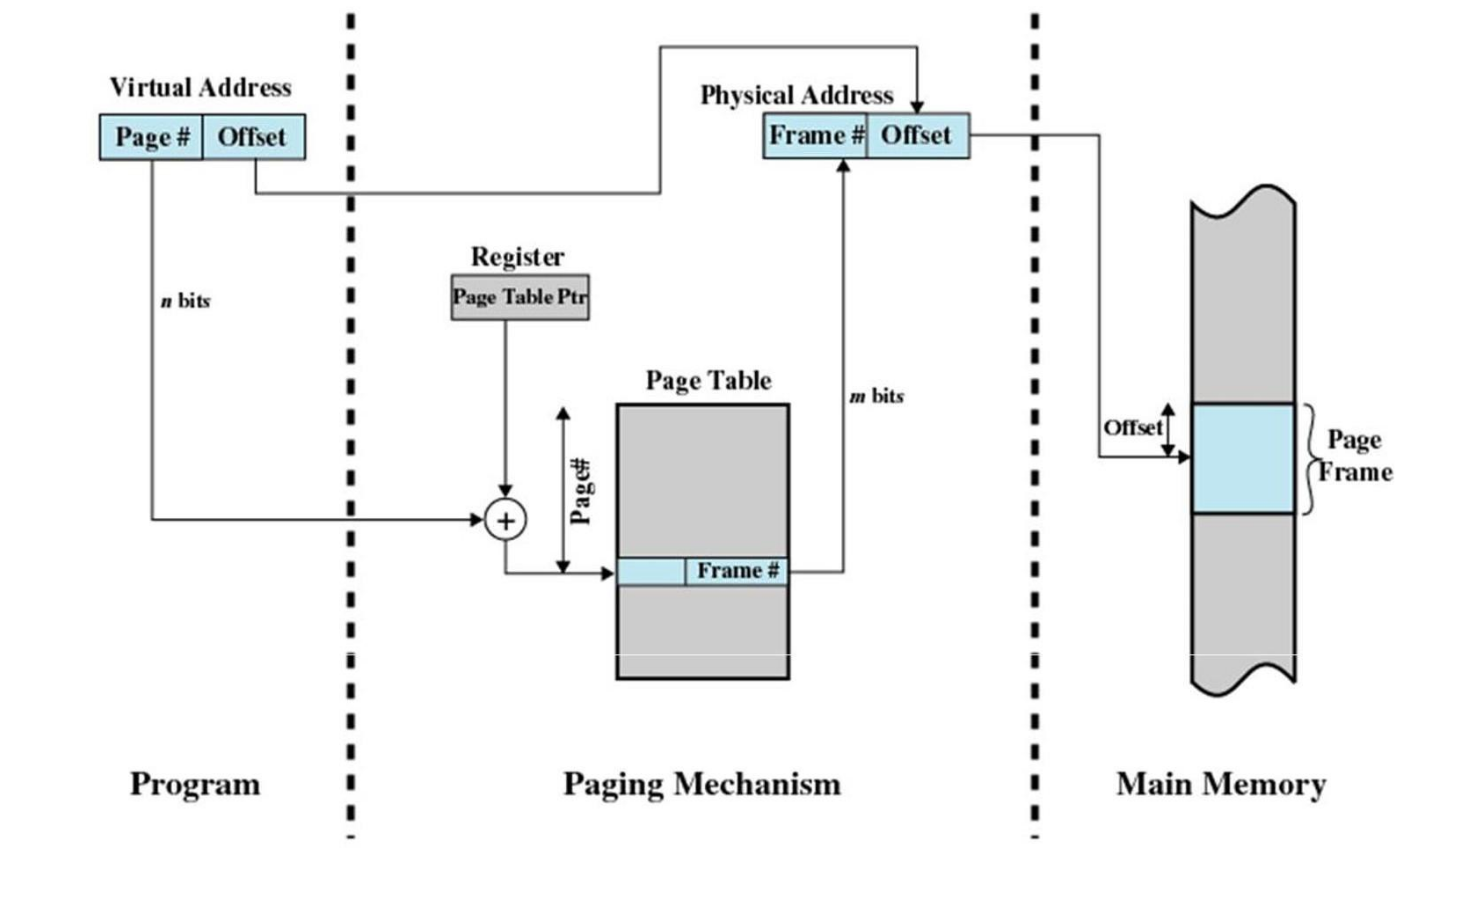
\includegraphics[width=0.80\linewidth]{Immagini/AddressMapping.png}
\caption{Descrizione grafica memoria virtuale.}
\end{figure}


\subsubsection{TLB (Translation Lookaside Buffer)}
Per velocizzare il multiplo accesso in memoria si usa una cache di indirizzi che si chiama Translation Lookaside Buffer (TLB), una piccola cache che contiene le entries della page table usate recentemente ed è direttamente nel processore.

\begin{figure}[!htb]
\centering
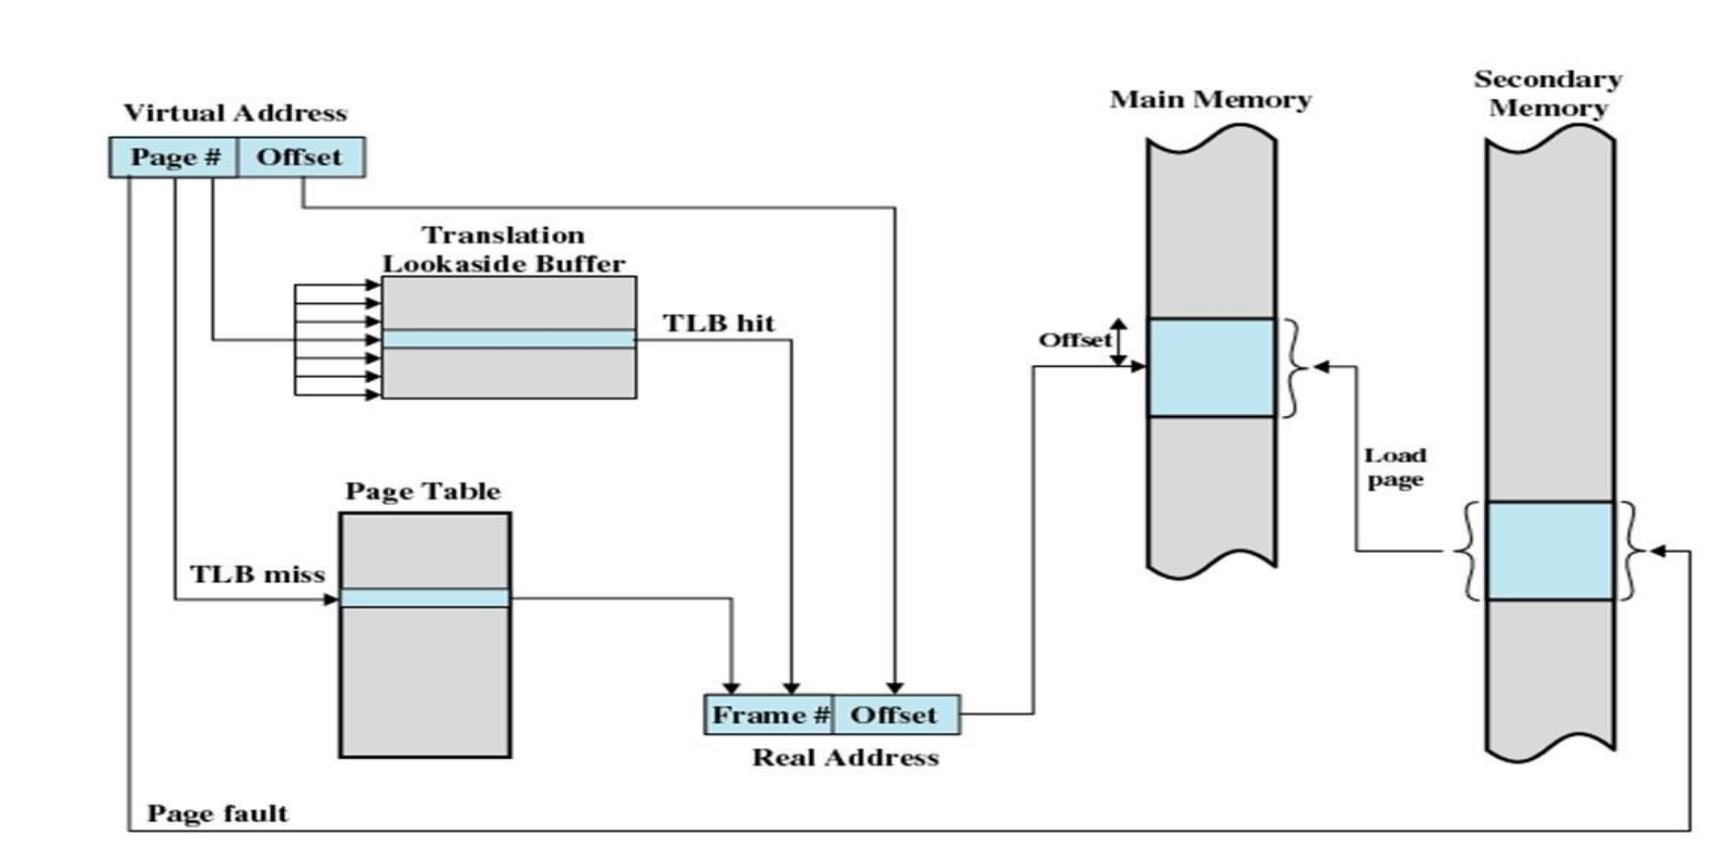
\includegraphics[width=0.80\linewidth]{Immagini/TLB.png}
\caption{Descrizione grafica memoria virtuale.}
\end{figure}

\newpage
\section{Codici di Controllo}
Per il controllo degli errori si usano dei bit di ridondanza della parola, per esempio una parola che viene memorizzata sul registro o sulla memoria inizialmente a \textbf{m} bit diventa una parola di codice di \textbf{n} bit con \textbf{n = m + r} essendo \textbf{r} i bit di ridondanza.

\begin{figure}[!htb]
\centering
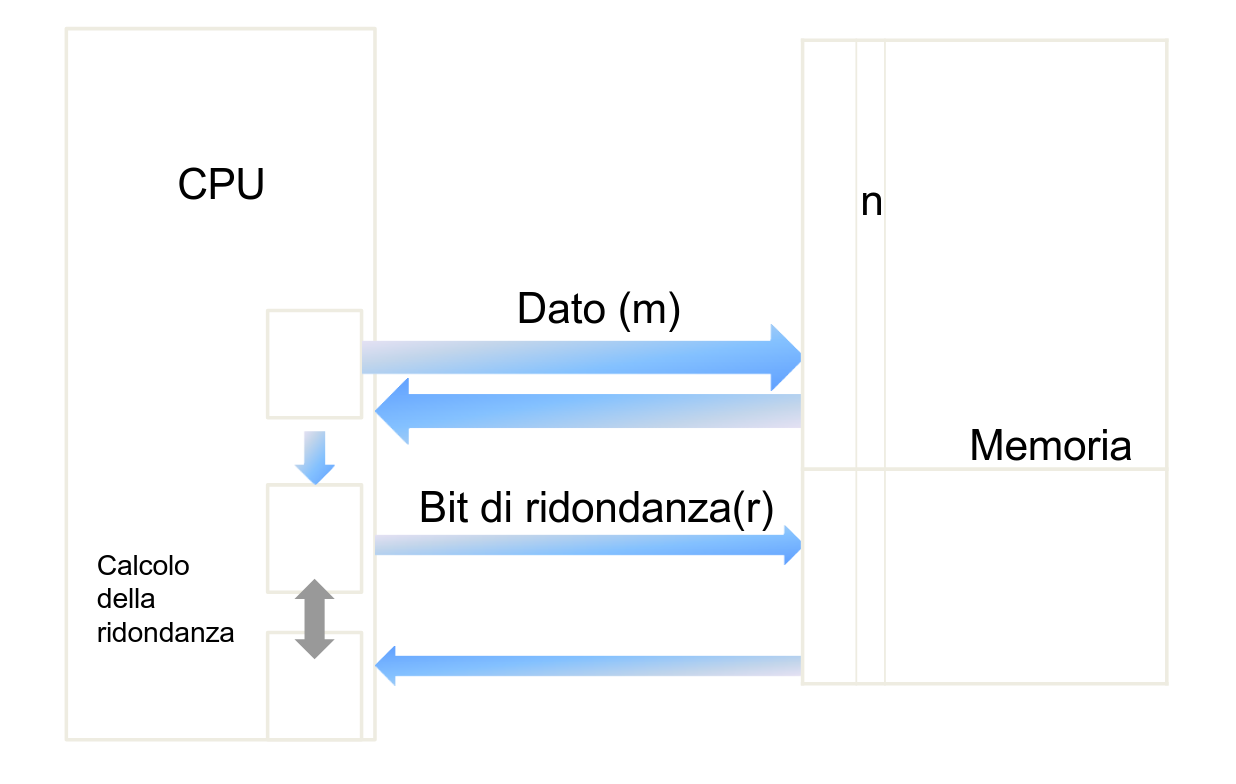
\includegraphics[width=0.65\linewidth]{Immagini/RamECC.png}
\caption{Esempio di bit di ridondanza nelle RAM ECC.}
\end{figure}

\subsection{Distanza di Hamming}
\hl{La distanza di Hamming tra due variabili binarie di n bit vale d (numero intero tra 0 e n) se d è il numero di cifre binarie diverse tra le due variabili.} Si calcola come: 
\[\text{EXOR: } d = \sum_{i=0}^{n-1}h_i\]
\begin{center}
\begin{tabular}{|c|c|c|}
    \hline
    $a_i$ & $a'_i$ & $h_i$ \\
    \hline
    \hline
    0 & 0 & \textbf{0} \\
    \hline
    \hline
    0 & 1 & \textbf{1} \\
    \hline
    \hline
    1 & 0 & \textbf{1} \\
    \hline
    \hline
    1 & 1 & \textbf{0} \\
    \hline
\end{tabular}
\end{center}

\textbf{NB:}
\begin{itemize}
    \item Se si vogliono rilevare k errori singoli è necessaria una parola con distanza d=k+1, perche’ con un codice di distanza k+1 non esiste modo che k errori singoli trasformino una parola valida in una altra parola valida.
    \item Se si vogliono correggere k errori singoli è necessaria una parola con distanza d=2k+1, perche’ in questo modo pur cambiando k bit la parola in codice sarà comunque più vicina alla parola originaria che a tutte le altre e quindi si può risalire alla parola originaria.
\end{itemize}

\newpage
\subsection{Codice di parità}
\hl{Il codice più semplice è il bit di parità (pari) che aggiunge 1 bit per fare in modo che il numero degli 1 nella parola sia un numero pari.}
Ha una distanza d=2 e quindi rileva solo 1 solo errore.
\textbf{ESEMPIO:} Progettare una rete che indichi se due ingressi binari sono entrambi uguali a zero, se il segnale d parità pari è corretto, altrimenti indichi errore.

\begin{figure}[!htb]
\centering
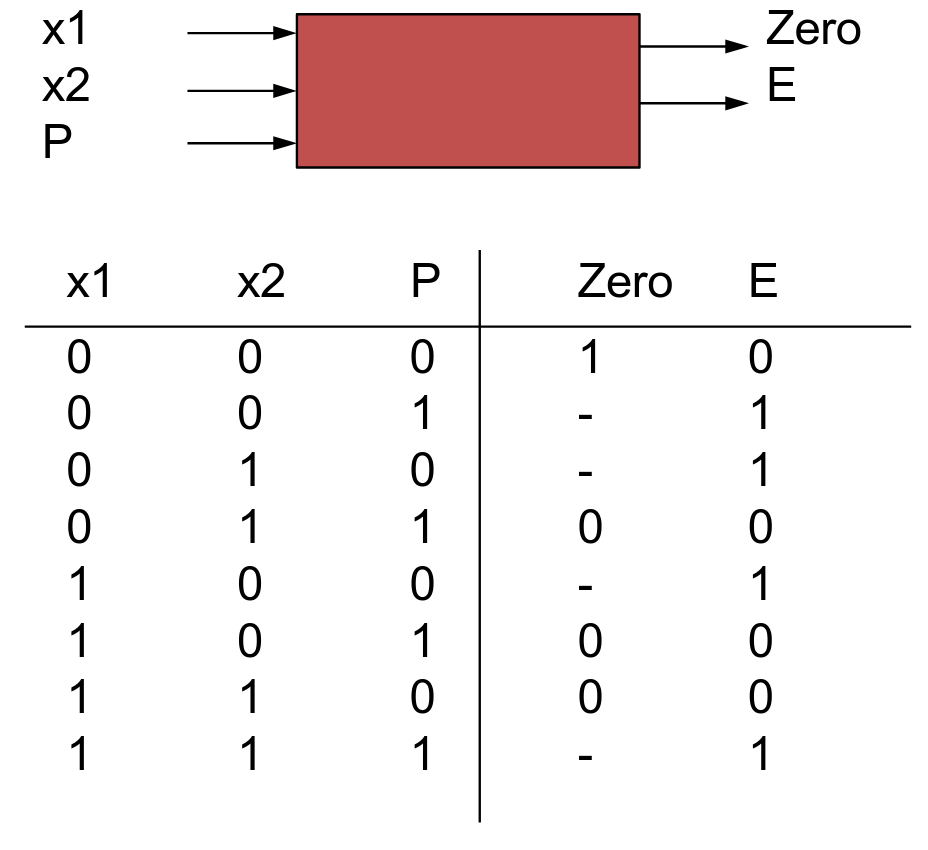
\includegraphics[width=0.40\linewidth]{Immagini/CodiceParita.png}
\caption{Esempio di codice di parità.}
\end{figure}

\subsection{Codice di Hamming}
\hl{Il codice di Hamming fornisce un algoritmo per generare codici ridondanti correttivi, tali che sia palese l’indicazione degli eventuali bit errati nella parola codice.}
Per ognuna delle $2^m$ parole legali codificate con n bit è necessario che il numero di parole sia:
\[2^n \geq 2^m (n + 1)\]
Così per ognuna delle $2^m$ parole legali che usano n bit si ha 1 parola giusta e n parole sbagliate ma vicine solo a quella legale:
\[2^r \geq m + r + 1\]

\subsubsection{Esempio: Esercizio con m=4}
Supponiamo di avere $m = 4$ bit, che sia \textbf{1011}.
\begin{enumerate}
    \item Trovare i valori della parola di n bit, dove $n = m + r$, con r che sono i bit di ridondanza. Dalla disequazione precedente sappiamo che per $m = 4$ abbiamo $r = 3$ e $n = 7$.
    \item Mettere i bit nella posizione corretta, nello specifico i bit di ridondanza dovranno essere messi in posizioni che sono potenze del 2. \textbf{NB:} Si parte da 1 e non da 0.
    \begin{center}
    \begin{tabular}{|c|c|c|c|c|c|c|}
        \hline
        $r_1$ & $r_2$ & $m_1$ & $r_3$ & $m_2$ & $m_3$ & $m_4$ \\
        \hline 
        \hline
        $b_1$ & $b_2$ & $b_3$ & $b_4$ & $b_5$ & $b_6$ & $b_7$ \\
        \hline
    \end{tabular}
    \end{center}
    Le $m_i$ sono i valori della parola originale, gli $r_i$ invece vanno calcolati.
    \item Per calcolare i valori $r_i$ è necessario creare due matrici:
    \[H = \begin{pmatrix}
            1 & 2 & 3 & 4 & 5 & 6 & 7\\
            \hline
            \cancel{1} & \cancel{0} & 1 & \cancel{0} & 1 & 0 & 1 \\
            \cancel{0} & \cancel{1} & 1 & \cancel{0} & 0 & 1 & 1 \\
            \cancel{0} & \cancel{0} & 0 & \cancel{1} & 1 & 1 & 1 \\
          \end{pmatrix}
    \] 
    H è una matrice $r \times n$ in cui vengono scritti in binario posizionati verticalmente i valori da 1 a n. E poi vengono cancellate le colonne corrispondenti agli $r_i$ per creare la matrice G.
    \[G = \begin{pmatrix}
            1 & 1 & 0 & 1 \\
            1 & 0 & 1 & 1 \\
            1 & 0 & 0 & 0 \\
            0 & 1 & 1 & 1 \\
            0 & 1 & 0 & 0 \\
            0 & 0 & 1 & 0 \\
            0 & 0 & 0 & 1 \\
          \end{pmatrix}
    \]
    G, invece, è la matrice creata a partire da H con le colonne cancellate. Nello specifico, per ogni colonna in ordine, se è cancellata vanno ricopiati i bit della riga che sono rimasti, se non è cancellata va copiata una riga della matrice identità.
    \item Per codificare il messaggio è necessario moltiplicare la matrice G per il messaggio m e fare modulo 2: 
    \[
        G \cdot m = 
          \begin{pmatrix}
            2 \\
            3 \\
            1 \\
            2 \\
            0 \\
            1 \\
            1 \\
          \end{pmatrix} 
        \text{modulo 2} =
          \begin{pmatrix}
            0 \\
            1 \\
            1 \\
            0 \\
            0 \\
            1 \\
            1 \\
         \end{pmatrix} 
    \]
    Quindi il messaggio codificato N è: 0110011
    \item Per controllarlo è sufficiente moltiplicare il messagio codificato N per la matrice H.
    \[
        m = H \cdot N = 
            \begin{pmatrix}
                1 \\
                3 \\
                2 \\
            \end{pmatrix}
        \text{modulo 2} = 
            \begin{pmatrix}
                1 \\
                1 \\
                0 \\
            \end{pmatrix}
    \]
    Quindi il bit trasmesso errato è il numero 011, ossia il numero 3.
\end{enumerate}


\section{Parallelismo}
\hl{Un’architettura parallela è un insieme di elementi di elaborazione che
cooperano e comunicano per risolvere velocemente problemi di dimensioni considerevoli,
talvolta intrattabili su macchine sequenziali.}
A livello di problema e di parallelismo computazionale si può definire il parallelismo:
\begin{itemize}
    \item \textbf{Disponibile (available parallelism)} nel programma o ancor meglio nell’algoritmo.
    \item \textbf{Utilizzato (utilized parallelism)} ottenuto durante l’esecuzione.
\end{itemize}
Compito dei calcolatori è cercare di rendere efficiente lo sfruttamento di tutto il parallelismo
disponibile in una applicazione, a due livelli:
\begin{itemize}
    \item \textbf{Parallelismo funzionale:} operazioni e parti delle soluzioni che possono essere eseguite nello stesso tempo.
    \item \textbf{Parallelismo di dato:} strutture dati e parti di esse su cui il programma può lavorare indipendentemente e nello stesso tempo.
\end{itemize}
Esiste una altra classificazione, che riguarda l’aspetto architetturale e che divide il parallelismo in due categorie:
\begin{itemize}
    \item \textbf{ Parallelismo Temporale (pipelining):} Un insieme di unità funzionali sono utilizzate in sequenza per realizzare una singola computazione.
    \item \textbf{Parallelismo Spaziale (Replicazione o parallelismo):} un insieme di unità funzionali sono replicate e utilizzate nello stesso tempo per realizzare una singola o diverse computazioni.
\end{itemize}
Una architettura parallela risolve due problemi:
\begin{itemize}
    \item \textbf{Speed-up:} lo stesso problema viene risolto in minor tempo.
    \item \textbf{Scale-up:} risolve un problema più grande nello stesso tempo.
\end{itemize}
\textbf{Scalabilità Forte (strong scaling)} misura l’incremento di velocità, mantenendo fissa la dimensione del problema ed aumentando hardware.\\
\textbf{Scalabilità debole (weak scaling)} l’incremento di velocità quando le dimensioni del problema crescono proporzionalmente alla crescita dell’hardware.
\\Ci sono 4 categorie di architetture:
\begin{enumerate}
    \item \textbf{SISD: Single Instruction Stream, Single Data Stream} singolo processori tradizionali con una unità di elaborazione e una unità di controllo.
    \item \textbf{MISD: Multiple Instruction Stream, Single Data Stream} sono le architetture in pipeline in cui un flusso di dati viene elaborato in cascata da istruzioni diverse in unità diverse.
    \item \textbf{SIMD: Single Instruction Stream, Multiple Data Stream} architetture con molte unità di elaborazione parallele che elaborano dati diversi con lo stesso flusso di istruzioni, gli array e i processori vettoriali.
    \item \textbf{MIMD: Multiple Instruction Stream, Multiple Data Stream} architetture composte da più unità di elaborazione più o meno lascamente connesse, ossia tutte le macchine parallele e distribuite attuali e le architetture multicore.
\end{enumerate}

\begin{figure}[!htb]
\centering
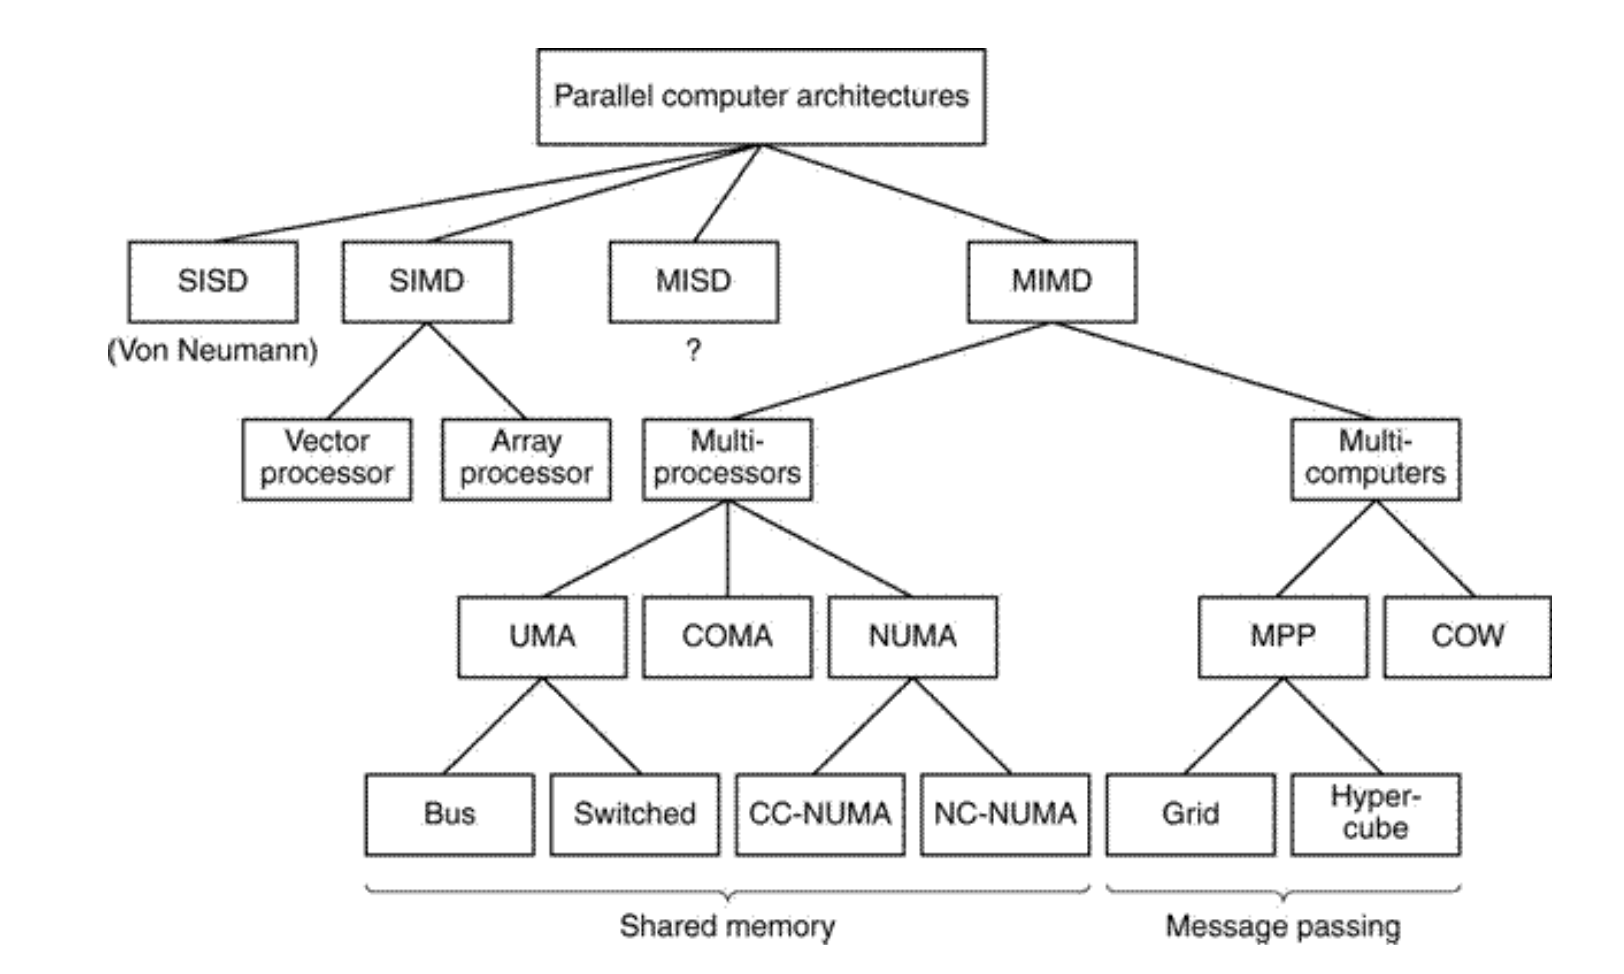
\includegraphics[width=0.70\linewidth]{Immagini/Architetture.png}
\caption{Tabelle delle architetture.}
\end{figure}

\subsection{Architetture MIMD}
L’architettura MIMD ha portato allo sviluppo di tutti i server paralleli, i cluster multi-lama e anche all’interno del chip alla realizzazione delle architetture Multicore, Many core.
\begin{itemize}
    \item \textbf{Multiprocessori (shared memory multiprocessors o SMP):} Replicazione di processori e di moduli di memoria condivisa con un global address space. Sono anche detti Shared -memory MIMD architectures perché lo spazio di memoria è condiviso tra tutti i processori e comunicano con variabili condivise e con meccanismi di sincronizzazione attraverso i diversi livelli di memoria. L’architettura è nata in genere per pochi processori e ora è la architettura di riferimento nei sistemi multicore e many core.
    \item \textbf{Multi-computer (distributed memory architecture):} Replicazione di PE (processing elements), come coppia processore/memoria, anche dette Distributed-memory MIMD architectures perché la memoria è distribuita e privata di ogni processore o message-passing MIMD architectures perché la comunicazione avviene con scambi di messaggi. I processori che lavorano in message passing come architettura parallela spesso usano un modello che si chiama SPMD Single Program Multiple Data, in cui di fatto i diversi processori eseguono lo stesso programma su dati diversi, ma permettendo un flusso di istruzioni diverso.
\end{itemize}

\subsubsection{UMA e NUMA}
Le architetture multi-processor possono avere gli accessi alla memoria secondo due metodologie:
\begin{itemize}
    \item \hl{\textbf{UMA (Unified Memory Access):} Ogni processore ha lo stesso tempo di accesso alla memoria.}
    \item \hl{\textbf{NUMA (Non Unified Memory Access):} Alcuni accessi sono più o meno veloci a seconda di quale processore richiede l’accesso.}
\end{itemize}


\subsection{Archittetura Multiple-Issue}
Archittetura studiata per avere un CPI $<$ 1 (oppure un IPC $>$ 1), è necessario far iniziare più istruzioni in un ciclo. 

\subsection{Archittetura Superpipeline}
Architettura in cui in ogni stadio molte operazioni sono eseguite in porzioni del clock
differenti. in questo modo  più istruzioni possono partire assieme (nello stesso clock) ottenendo quindi un CPI $<$ 1.

\subsection{Archittetura VLIW (Very Long Instruction Word)}
Architettura che almeno in alcune operazioni, esegue un numero fissato di istruzioni $>$1 , con più unita funzionali in parallelo. Tali istruzioni sono formattate in una sola istruzione in modo staticamente determinato dai compilatori. Questa è una scelta definita della ISA e realizzato dal compilatore al tempo di complazione.

\subsection{Archittetura Superscalare}
Architettura progettata per eseguire un numero variabile di istruzioni contemporaneamente in unita’ funzionali diverse, decise in modo dinamico. La scelta di quali istruzioni eseguire dipende dall’unita’ di instruction fetch che:
\begin{enumerate}
    \item Acquisice piu’ istruzioni assieme..
    \item Verifica se alcune istruzioni possono essere eseguite su unità funzionali diverse e disponibili.
\end{enumerate}
L’impiego efficiente è ottimizzato dai compilatori che mettono vicine istruzioni che non hanno dipendenze o anti-dipedenze. È perciò una scelta di microarchitettura.

\subsection{Esecuzione Speculativa}
Lo scopo primario è di non porre in stallo la pipeline cercando di evitare le alee RAW e le alee WAW e WAR in caso di multiple pipeline.
\hl{Si dice \textbf{Esecuzione speculativa} se l’esecuzione di un blocco avviene prima di sapere se il blocco deve essere eseguito.}
È necessario il supporto sia del compilatore che di hardware dedicato.
I risultati vanno in registri temporanei, gli scratch register, che poi vengono copiati sui registri veri solo se il blocco doveva davvero essere eseguito.
Esiste una tabella che tiene traccia di che blocco è eseguito o è in esecuzione.

\subsubsection{RAT (Register Alias Table)}
Avviene quindi internalmente una rinomina dei registri in scratch register che è necessaria sia per non modificare i registri veri e sia per evitare alee di tipo WAW e WAR quando più unità lavorano in parallelo e in più pipeline.

\subsubsection{Fuori Ordine}
La soluzione seguente permettere una esecuzione fuori ordine, dove ogni blocco può essere eseguito anche non nell’esatto ordine deciso dal programmatore e dal compilatore, con i soli vincoli che:
\begin{itemize}
    \item I dati vanno prelevati in ordine (in-order issue).
    \item I dati vanno riscritti in ordine alla fine (in-order commit).
\end{itemize}

\subsection{Interrupt e Polling}
La gestione degli eventi e della comunicazione con I/O può creare delle interruzioni e può essere gestita in due modi:
\begin{itemize}
    \item \textbf{Polling:} Il metodo piu’ semplice, a controllo di programma con interrogazione periodica. La CPU verifica lo stato della periferica, continua la richiesta fino a che non verifica che e’ pronta per ricevere dati in uscita o fornire dati in ingresso e poi eventualmente inizia il trasferimento dati. Se necessario, ricomincia.
    \item \textbf{Interrupt:} Sospensione forzata del processo di esecuzione e trasferimento di controllo ad una routine di servizio (ISR) che soddisfa le richieste dell'evento che ha provocato l'interruzione, al termine della quale il controllo viene restituito al processo sospeso.
\end{itemize}

\subsubsection{Interruzioni}
Le interruzioni possono essere di due tipi:
\begin{itemize}
    \item \textbf{Sincrone:} sono dette anche eccezioni e sono dovute al programma e sono di due tipi:
    \begin{itemize}
        \item \textbf{Processor-detected exception.}
        \item \textbf{Programmed exceptions.}
    \end{itemize}
    \item \textbf{Asincrone:} sono di tipo hardware e derivano da sorgenti esterne come da periferiche di I/O e non sono relative all’istruzioni che si stanno eseguendo.
\end{itemize}

\subsubsection{Fauls}
Le faults sono istruzioni che non si devono eseguire, come ad esempio eseguire una istruzione senza avere i privilegi, o scrivere in una parte read only. Sono riscontrate prima di incrementare il program counter e bloccano il programma. L'istruzione successiva non viene eseguita.

\subsubsection{Traps}
Le traps sono dovute disolito al debugger e sono una chiamata ad un programam che è la funzione del debugger, sono eseguite dopo aver incrementato il PC e poi il programma va avanti. Le trap anomalie di funzionamento rilevate e gestite immediatamente dopo dell'esecuzione dell'istruzione che le genera.

\subsubsection{Aborts}
Le aborts anomalie di funzionamento che non permettono di individuare esattamente l'istruzione che le hanno determinate: ad esempio un malfunzionamento segnalato da una periferica.


\end{document}
